\subsection*{Jueves 25 de Agosto -- Kassel -- 80~km}

Comentario al pie pero arriba: \textquestiondown d\'onde se ha visto un cyber
que no venda chocolates? \textquestiondown Pueden creer que no existen los
alfajores? \textexclamdown De las cosas que se ocupa el pensamiento (estomacal)
mientras escribo!\\

Gustavo me despert\'o despu\'es de preparar un buen chocolate caliente,
riqu\'isima malcrianza. Prepar\'e el equipaje, y sal\'i. Mientras miro las fotos
de la camarita recuerdo c\'omo en esos momentos pensaba ``\textquestiondown
c\'omo ser\'a?'', y al ver las siguientes fotos veo lo excelente que fue y es.

Empez\'o este primer d\'ia no tan bueno, con clima muy nublado, lluvias
pasajeras que me hac\'ian morir de fr\'io, y viento en contra. Alargu\'e mucho
el viaje a Kassel: \textexclamdown 80~km! Fui por el camino que hicimos con
Gustavo (esta vez no me perd\'i) y me hizo pensar en lo bueno de perderme la
primera vez, que volv\'i moribundo del cansancio a G\"ottingen. Llegu\'e bien,
bien cansado por el viento en contra pero temprano y con alimentos para
reponerme.

Baj\'e a Kassel bordeando el r\'io, es la \'unica parte del viaje que era nueva
para m\'i en bici. Desde arriba en los bosques (donde se cay\'o la mochila de la
bici, que llevo ahora en la espalda) hasta el r\'io tuve interesantes curvas en
bajada, aunque mojadas. Par\'e en un gran \'arbol que reparaba de la lluvia
mirando andar al ferry, y abr\'i la mochila para aspirar algo. \textexclamdown
Encontr\'e todo cubierto por chocolate rayado! Gustavo envolvi\'o las sobras del
desayuno, y se rompi\'o el papel de aluminio que lo guardaba. Lo primero que
com\'i, claro est\'a. \textexclamdown Cada vez que uso la toalla quedo con un
perfecto aroma a chocolate! Mejor que el que traigo seguro: a diferencia de los
7 lagos o Mendoza (\textquestiondown de qu\'e depender\'a?) ac\'a apesto.

Compr\'e panes con semillas en una \emph{B\"ackerei}. \textexclamdown Qu\'e
ricos son! La encontr\'e por cambiar de camino, casi llegando a Kassel. Se
ve\'ia a lo lejos el H\'ercules Me atendi\'o una mujer joven divina, a
diferencia de todo el mundo no hablaba ``a little bit'' ingl\'es, porque lo
hablaba, decididamente. Tambi\'en com\'i barritas energ\'eticas, regalo de Ina,
riquis\'isimas. Le pregunt\'e a esta mujer por Hostales. Me indic\'o uno a 6 km
que hacen descuentos a ``cyclers'' pero\ldots\ \textexclamdown volviendo! Me
pregunt\'o si quer\'ia que buscara ella en la gu\'ia y le dije que no, menos mal
que insisti\'o. \textexclamdown Vaya uno a saber qu\'e se me cruz\'o por la
cabeza al negarle este salvataje urbano! Consigui\'o una direcci\'on, y
despleg\'o un mapa de Kassel en una mesa mientras me comentaba que algo que las
mujeres no saben hacer, es abrir mapas; y no paraba de hablar. \textexclamdown
Yo mor\'ia de risa! Pero no le cont\'e sobre mis dilemas abriendo mapas. Me
ense\~n\'o c\'omo llegar. No contenta con eso escribi\'o la direcci\'on y
nombre, a Dios gracias tambi\'en. Como ac\'a no existen las manzanas y
urbanizaci\'on planificada como la conocemos, fue un l\'io llegar. Preguntando
lo encontr\'e. Casi todos muy amables.

El lugar es de una organizaci\'on de alojamiento juvenil de Alemania que m\'as
bueno no puede estar. Y en relaci\'on euro, barato. \textexclamdown L\'astima
que traje un numero de euros tambi\'en en relaci\'on euro! Muy buena onda, me
guardaban la bici, buenas duchas (croto es el que quiere, no el que viaja en
bici ac\'a), s\'abanas, tel\'efono y desayuno. Piezas compartidas, duchas
compartidas entre piezas\ldots\ todo el lujo que a un joven viajero no le debe
faltar. En realidad al tel\'efono podr\'ia sacarlo de la lista de facilidades:
en un hall que retumbaba, y escup\'ia todas las monedas\ldots\ \textexclamdown
Para colmo me las quer\'ia sacar de encima! Me llev\'e una buena impresi\'on,
aunque parar durante un mes, por baratos que sean, es un presupuesto, tal vez
necesario. \textexclamdown Mi traste decidir\'a!

Me pregunt\'o la joven recepcionista (de mi edad, o por ah\'i) si prefer\'ia
hablar en espa\~nol. Le dije, todav\'ia en ingl\'es (cambiar se me complica
m\'as que pensar), que me daba igual, pues: ``\emph{I'm from Argentina}''.
``\textexclamdown Me est\'as jodiendo!'' contest\'o sonriente, en
argentin\'isimo. Agreg\'o que vivi\'o 5 a\~nos en Argentina, con su familia
supongo de Alemania. \textexclamdown Como ven, cada vez me sent\'ia mas
inc\'omodo! Todo arreglado y sobre ruedas: me dej\'o una lista con todos los
hosteles de Alemania, preguntando si quer\'ia los de Europa tambi\'en.

Llegu\'e a mi pieza. Com\'i casi todo lo que quedaba en la mochila, menos el
buzo polar amarillo que estaba muy sucio. La ducha pegaba fuerte
masajeando, y quemaba. El para\'iso: en vez de dejar abierta la caliente y la
fr\'ia hasta donde este pollo de incubadora permita, regulaba presi\'on y
temperatura. \textexclamdown Por \'unica vez en mi vida, qu\'e vivencias y
lujos que uno tiene de viaje!

El tema es que la panadera y sin saberlo me organiz\'o para todo el viaje un
tema no menor: d\'onde dormir. Espero ma\~nana haya sol para darle con m\'as
ganas.\\

Kassel es una ciudad muy oscura de noche, le da el romanticismo de ``Lisa
Simpson'' para el turista que puede ver el cielo, aunque no es de lo m\'as
c\'omodo para caminar. Sin embargo en la noche est\'a oscuro de verdad, no
como en Buenos Aires que entra luminosidad por las ventanas, y no se ven las
estrellas.

\subsection*{Viernes 26 -- Casi Marburg (casi, \textexclamdown por 45~km!) --
80~km}

Dorm\'i hasta las 6 am, hora en que abren la cafeter\'ia para el desayuno.
Como mis intervalos son de media hora al despertarme, repos\'e de nuevo
tranquilo, levant\'andome nada menos que a las\ldots\ \textexclamdown 7:42 am!
\textexclamdown Pero esto es \emph{doce} minutos despu\'es de que cierre! (Uno
se contagia de las culturas en las que vive, che). Menos mal que fue todo un
gran susto, porque cuando baj\'e verifiqu\'e que segu\'ia abierta. Y suerte que
en el apuro olvid\'e las medias, pero no el pantal\'on. Qu\'e desesperado por un
desayuno, es que es por lo que justifico pagar alojamiento. Viajando en bici no
es un tema menor el buen alimentaje.

Cuando vi que era \emph{self-service} me convert\'i en ardilla que copiaba
r\'apidamente todo lo que hac\'ia quien estaba delante m\'io, tambi\'en
despertada vergonzosamente tarde. \textexclamdown Como no sab\'ia lo que
hac\'ia termin\'e comiendo cereales con yogur y con leche! No est\'a nada mal,
ver'an.

Mientras devoraba entraba una familia disfrazada de ciclistas. A padre, madre
e hijo les faltaba entrar con el casco puesto para completar la imagen. Me
levant\'e para preguntarles qu\'e hac\'ian, y esperaba que me contestara
``viajamos en bici'', pero pacientemente me dijeron que iban de
no-se-qu\'e-pueblo a no-se-qu\'e-otro-pueblo. M\'as concretamente para m\'i,
de la Selva Negra a los lagos del norte; este tipo s\'i que se eligi\'o bien
esposa e hijo. Me dijo que me esperaba un buen viaje siendo que voy al lugar
desde donde ellos salieron. ``Gracias, \emph{Guten fahren}!'' en mi alem\'an
indio. Lo dije al recordar lo que me dijeron otros ciclistas al irme del
\'arbol del ferry: ``\emph{Guten fahr}''. Buena onda, aunque no divinos como
esperaba. Al visitar otros hosteles vi que est\'a lleno de viajantes en bici,
no es cosa de andar charlando con todos al levantarse a desayunar.

Ahora a armarme las valijas y tomarme la pr\'oxima bicicleta direcci\'on
Sudoeste. \textexclamdown Viva el sol!\\

Empec\'e puteando, porque no sab\'ia c\'omo salir de Kassel. Mucho menos hacia
d\'onde, exactamente. \textexclamdown Son tantos los caminos, pero tambi\'en
tantos pueblos! \textexclamdown Y d\'onde cornos est\'a la salida de esta gran
ciudad! Cuando cruc\'e esa avenida que sube al H\'ercules se ve\'ia, dos
cuadras arriba, l\'io de polic\'ias y gente. Sin interesarme segu\'i camino
por donde uno de los tantos transe\'untes me hab\'ia indicado. Era en subida,
y al poco tiempo los polic\'ias y un Mercedes clase A con calcos se acercaban,
lentamente. Yo iba m\'as lento, pedaleando dubitativo. Le pregunt\'e a un
polic\'ia en moto {\small BMW} c\'omo salir a tal pueblo, y aunque quiso no
pudo ayudarme; ven\'ia atento mirando a atr\'as, y cuando lo acompa\~n\'e
mirando, la sorpresa: \textexclamdown numerosos ciclistas --m\'as de 200
seguro, pero no quiero aproximar n\'umeros grandes-- en caravana! Bicis y
gente de todo tipo pero un color: \textexclamdown las que no hablar\'an otro
idioma que no sea el alem\'an! Las calcos del Mercedes indicaban un circuito
en bici. Sal\'ian justo hoy desde Kassel, para andar el fin de semana en
los alrededores. No sab\'ia que hacer\ldots\ estaba cerca del H\'ercules, de
perderme, de seguir mi camino y tambi\'en de seguirlos a ellos. No sab\'ia a
d\'onde iban, pero unidos ser\'ia mejor que hacer mi trayecto (aunque bien)
solo.

As\'i que ya en el mal\'on, me acercaba a cada deportista para preguntar si
hablaba ingl\'es, y entonces a donde \'ibamos; pero el \'unico joven que me
contest\'o a la primer pregunta con un ``s\'i'', remat\'o luego con un ``no
s\'e''. \textexclamdown Estoy nervioso! Pero me auto-convenc\'ia de que si me
tranquilizaba ser\'ia m\'as divertido que andar solo, as\'i que eso hice. De
todos modos con mi instinto ``indio de las pampas'' supe que iban al sur,
porque bordeaban el r\'io, en sentido contrario al de la corriente, y me
acercar\'ia a Heidelberg. S\'olo lament\'e que no pararan en un cementerio de
la II Guerra Mundial, hecho monumento.

A los 30~km, cerca de Felsberg, paramos y por fin esta buena se\~nora hablaba
ingl\'es. Ten\'ia una de las mejores bicis sino la mejor, estilo todo terreno
pero ``agresivo'', no bici de monta\~na t\'ipica. Frenos a disco, todo {\small
XTR}, doble suspensi\'on\ldots\ \textexclamdown ``\emph{This is my baby}'', la
present\'o! La sorpresa porque esta jugadora de tenis que supo nombrar a
Sabattini ronda los 80 a\~nos, cuentas que cierran al calcular que hace 60
a\~nos termin\'o la escuela. Pedalea 6.000~km anuales por Alemania.
Una buena onda terrible. Y juventud. Mostr\'andome en un mapa d\'onde queda
Felsberg (y notific\'andome que efectivamente ah\'i est\'abamos, o cercanos)
confirm\'o mis rudimentarias orientaciones. Era camino directo al sur, y yo me
hubiese desviado al este para conocer un lago. Cre\'ia estar m\'as cerca de
Marburg y me cost\'o un gran cansancio el intentar llegar. Luego me explic\'o
el camino del circuito y para mi sorpresa me un\'i a la \'unica etapa que me
acerca a mis destinos. Luego van en direcci\'on Oeste, Norte y Este.
\textexclamdown Se supone si es circuito!

Dejamos las bicis y subimos unas cuadras a buscar almuerzo. \textexclamdown Yo
segu\'ia tanto a todos lados a mi angelito de la guarda que casi entro al
ba\~no de mujeres! Us\'e el ba\~no de al lado, luego ser\'ia f\'acil
rastrear a esta mujer: pelo blanco y corto, y remera de \emph{Specialized} de
tantos colores que no los recuerdo, pero todos chillones.

Por el pueblo hab\'ia bailes y vestimenta t\'ipica de Alemania, dos caballeros
medievales caminando forzadamente\ldots\ \textexclamdown cuando los llamaban
para una foto y se daban vuelta, mov'ian todo el torso primero, para
acompa\~narlo luego por piernas y caderas, incomodidad absoluta esas armaduras.
Mesas organizadas tipo las colectividades de la Rural, con muchos lugares donde
comprar alimentos tipo las colectividades, pero con un solo pueblo t\'ipico
representado: el alem\'an. Compramos unos fideos a la bolognesa con ensalada
alemana, todo buen\'isimo para andar mucho en bici. \textquestiondown El precio?
\geneuronarrow{4,5}. \textexclamdown Sin saber c\'omo salir de Kassel, un
mal\'on me llev\'o de la oreja por mi camino, ahora com\'ia barato alimentos
especiales para ciclistas, y luego conoc\'ia un castillo que no estaba en mis
planes! Y a una mujer que de anciana s'olo ten'ia la edad, y contagiaba ganas de
hacer deportes. Ni en sue\~nos todo esto.

Bien nutrido conoc\'i el castillo, donde un gu\'ia charleta en alem\'an
me aburri\'o as\'i que me dediqu\'e a mirar vistas y esas cosas, que en este
``simple'' castillo era lo que m\'as gustaba. La flecha de la veleta en lo
alto de una torre indicaba exactamente a donde yo iba. De all\'i ven\'ia
el viento, que dentro del pelot\'on no hab\'ia sentido por 30 kil\'ometros.
Desped\'i a la se\~nora, y me prepar\'e para seguir viaje.

Entr\'e en un ba\~no para cargar agua. Un alem\'an mediante se\~nas no me
dej\'o, indic\'andome la ``\emph{wasser station}'' a la entrada del pueblo,
donde dejamos todas las bicis. Llegu\'e y se trataba de un cami\'on lleno de
bebidas energ\'eticas. As\'i que adem\'as ahora ten\'ia agua con minerales y
mejor sabor que el de mi botellita pl\'astica.

\textexclamdown Ya era un d\'ia completo! Pero faltaba rebalsarse.\\

Camino a Marburg el viento me termin\'o parando en seco, por suerte.
\textexclamdown C\'omo me enoja el viento! Cambia en 20~km/h la velocidad
promedio, y en buena medida el cansancio y tiempo sentado en sill\'in. Maldito
cambio de clima: nublado con una peque\~na llovizna. Tom\'e medio mal un
camino de 5~km (en este viento significaba m\'as tiempo que distancia) y
llegu\'e a una antigua granja. El joven granjero de muy buena onda me indic\'o
en mi mapa el camino, pero al ver que no era lo suficientemente detallado fue
a la camioneta a buscar el suyo. Me mostr\'o que la ruta que hab\'ia
escogido no era tan buena para bicis, y que sub\'ia y bajaba muchas colinas,
as\'i que deber\'ia volver a tomar la otra ruta. Su insistencia se notaba por
querer ayudarme, as\'i que logr\'o que volviera. Me tragu\'e los 5~km a
40~km/h por el viento ahora a favor, y luego de costado/en-contra me hizo
frenar en un cartel de camping.

En este pueblo los mismos carteles se contradec\'ian, y nadie me supo explicar
d\'onde era el lugar donde podr\'ia usar mi bolsa de dormir. Hotel caro para
m\'i, y feo. Decid\'i parar totalmente media hora, y comer barritas en un
banco de plaza para luego seguir. Un muchacho con auto nuevo iba y ven\'ia a
fondo, el primer y \'unico ``nervioso'' manejando que vi en todo este viaje.
Pens\'e en pedir alojamiento en cualquier galp\'on, pero tambi\'en pens\'e en
que si sal\'ia 4:30 pm, en 4 horas, podr\'ia completar los 55~km a
Marburg; triste sue\~no, me dol\'ia hasta la espalda.\\

Volv\'i a frenar a los casi 15~km, en Schwalmstadt (parte de la \emph{Fachwerk
stra\ss e} alemana). \textexclamdown Es tan hermoso, que me alegr\'e de parar
y todo! Un hombre me supo indicar una \emph{Gasthaus}, al llegar vi que
abr\'ia en media hora. Llegu\'e acompa\~nado de unas muchachas, porque me
hab\'ia pasado, y como se les complicaba explicarme en ingl\'es, me hicieron
se\~nas de que las siguiera. Ayudar parece ser un deber. Una mujer que andaba
por ah\'i me indic\'o un tel\'efono a 500 m, as\'i que dej\'e la bici
esperando en la \emph{Gasthaus}, y camin\'e a buscarlo.

\textexclamdown Qu\'e lindo pueblo! Todas casas \emph{Fachwerk}, todo antiguo
y bien mantenido, todo bello y todo t\'ipico. Dos planeadores me sobrevolaban
en silencio. \textexclamdown Cuando estaban cerca me daban la misma impresi\'on
que las turbinas e\'olicas! Pas\'e de largo el tel\'efono, por supuesto.

Entr\'e en un parque central, y hab\'ia casas a\'un m\'as bellas, la iglesia
principal y un comercio. Entr\'e a preguntar por el tel\'efono. La mujer
sali\'o, y me acompa\~n\'o hasta poder se\~nalarlo.

\subparagraph{}\label{ssub:oficinaDeTurismo} --- \textquestiondown De d\'onde
sos? -- Pregunt\'o mientras.\\ --- De Argentina.\\ --- \textquestiondown Y
cu\'anto tiempo te quedar\'as por aqu\'i?\\ \hangindent=1cm

Y otras preguntas por el estilo me hicieron notar que no se trataba de un
comercio, sino de Informaci\'on Tur\'istica. Antes de llamar decid\'i
aceptar su ayuda (noten que deb\'ia aceptarla, no pedirla), porque no
conoc\'ia a las \emph{Gasthaus}. Eran caras pero no importaba, estaba
cansad\'isimo. Para confirmar que hubiera lugar, me mand\'o a otra 4~km hacia
el sur. Us\'o mucho el tel\'efono y al confirmar esta pensi\'on empez\'o a
preguntar: ``\textquestiondown Caf\'e o t\'e? \textquestiondown Qu\'e com\'es
con el desayuno? \textquestiondown Y a qu\'e hora?'' Y es que no era algo
p\'ublico: eran habitaciones privadas, y me di cuenta al entrar m\'as tarde en
la hermos\'isima casa. Firm\'e un agradecimiento castellano en el libro de
visitas, llev\'e algunos folletos tur\'isticos, busqu\'e mi bici, y volv\'i al
tel\'efono p\'ublico.\\

Llam\'e a Gustavo fascinado de tantas coincidencias buenas. Me record\'o
la frase del Alquimista: ``Cuando uno se propone realmente algo todo el
universo se torna para ayudarlo''. No me suena convincente, pero se est\'a
cumpliendo. Mi hermano agreg\'o una elogiosa y menos metaf\'isica frase:
``Nunca hay viento a favor para quien no sabe a donde va''. \textexclamdown
Nada de andar tom\'andolo literalmente, claro! Hab\'ia cena en casa de Gustavo,
y no me olvido de su emoci\'on al escuchar tantas buenas noticias juntas. En
realidad, como siempre, me puse euf\'orico mientras hablaba; \textexclamdown
seguro exager\'e todo!

Antes me dol\'ia cada pedaleada, y ahora que sab\'ia d'onde iba a dormir y
estaba contento de conocer algo que no estaba en planes, no sent\'ia el viento
si es que todav\'ia quedaban vestigios despu\'es del derroche. El sol volv\'ia a
salir y dejaba ver la cantidad de rutas que dejan los aviones, uno disfruta
tanto de ver el claro cielo al viajar pedaleando. La mujer de info tur\'istica
lo anunci\'o para ma\~nana (no le err\'o). \textexclamdown Y al ver mi sonrisa
lo asegur\'o tambi\'en para toda la semana!

Llegu\'e mal a la ``\emph{Privat Pension}'' (\textexclamdown obvio!) y esta
due\~na de casa me acompa\~n\'o hasta donde era. Yo no pod\'ia creer que no
tuviera carteles, pero claro, no es \emph{Gasthaus}. Lo dud\'e un poco, y entre
los timbres encontr\'e ``\emph{Albrecht}''. Al menos estaba.\\

Me atendi\'o un flaco de barba, muy flaco al menos de cara. Al entrar me
recibi\'o tambi\'en un gran afiche: un mapa de Alemania cruzado por una
diagonal de Nordeste a Sudoeste, con 12 puntos similarmente espaciados; al
lado, una nota del diario con foto de este mismo hombrecito corriendo:
``\textexclamdown 1.200~km en 12 d\'ias!'' 5 de descanso parece que tiene, en
promedio 80~km/d\'ia tiene que dar. \textexclamdown Era \'el! Lo mir\'e
incr\'edulo, y se re\'ia. El guacho habla s\'olo alem\'an, pero ten\'ia tanto
inter\'es como yo por comunicarse as\'i que en ingl\'es-alem\'an y muchas
se\~nas charl\'abamos. El poco tiempo que estuvo su amigo sirvi\'o de
int\'erprete.

La casa es hermosa. El tipo hace masajes y alquila habitaciones,
tiene 5 camas pero en mi gran habitaci\'on hab\'ia s\'olo una. Es a la
antigua: tengo cama, espejo, todo madera, mesa circular central, silla al lado
de la cama, mesita contra la ventana con m\'aquina de escribir, cuadros y
retratos\ldots\ a la antigua belleza. Una de sus pocas preguntas:

\subparagraph{}\label{ssub:rauchenSie} --- \textquestiondown Fum\'as?\\ ---
No.\\ --- Perf\'ect. -- respondi\'o, se\~nalando dos carteles que invitaban a
no fumar, pero no el cl\'asico pucho tachado sino otros m\'as bonitos.\\
\hangindent=1cm

La puerta de atr\'as da a una galer\'ia de madera, c\'alida y bonita, que a
pesar de la ciudad solo tiene vista a \'arboles. Muchos adornos, y creativos,
por ejemplo: un sill\'on colgado de dos cadenas es en realidad un yugo. S\'olo
desentonaba una hermosa l\'ampara de cristal; no combinaba con el estilo
r\'ustico. Trofeos y afiches sobre pedestrismo por doquier. Sobre una mesita
rodeada de dos bancos largos comunes y tres sillas con ornamentos en madera,
una botella redonda de vino tinto franc\'es, y copas de barro adornando sus
costados. Parece una descripci\'on de una novela medieval, pero se trata de la
casa donde pas\'e la noche. Recordar las casualidades que se unieron para que
termine en esta casa me emociona. Justo la de un hospitalario mega-maratonista.

\begin{center} 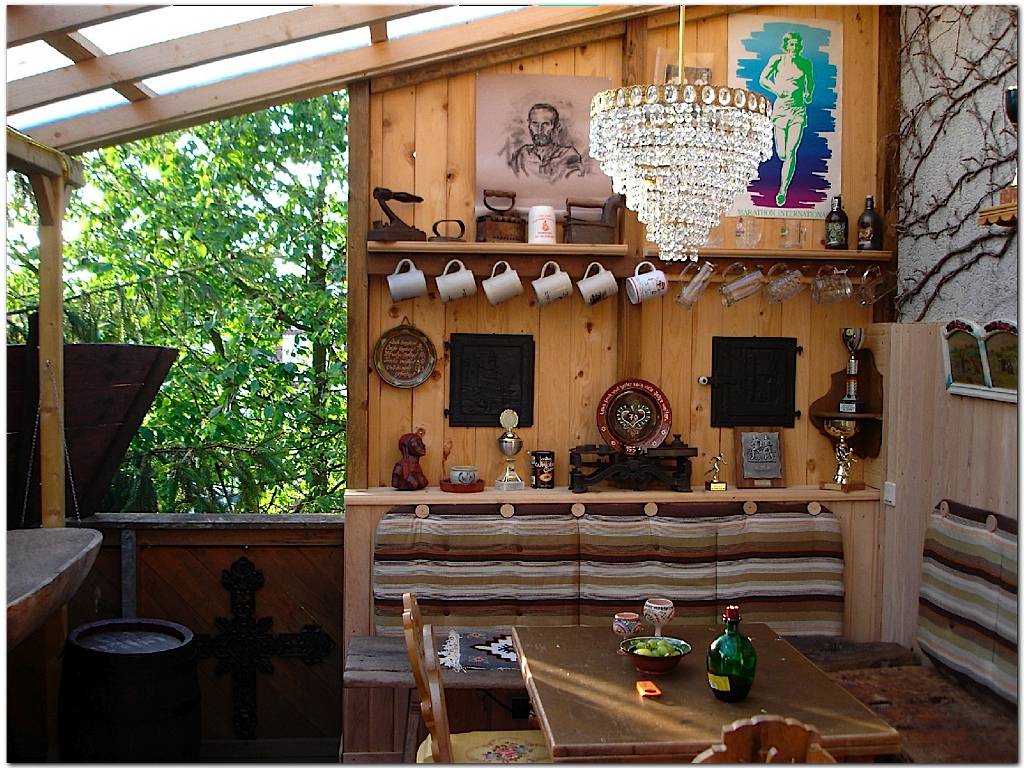
\includegraphics[width=300px]{images/DSC01605.JPG}\\
\textsc{Galer\'ia de la casa del maratonista.} \end{center}

Me di un ba\~no, orden\'e, y pens\'e en escribir en aquella mesita de afuera
pero ten\'ia hambre. Justo sal\'ian a la galer\'ia, as\'i que pregunt\'e por
una panader\'ia. En 500m me perd\'ia cuatro veces seg\'un su explicaci\'on,
as\'i que desist\'i de comprar pan terminando con las sabrosas barritas
energ\'eticas. Me invitaron a un vino, y charlamos sobre correr y el deporte.
Contaban que la galer\'ia era nueva, para festejar su cumplea\~nos en 12
d\'ias.

\subparagraph{}\label{ssub:queEdadTenes} --- Cuarenta. -- dijo el amigo.\\ ---
Gran fiesta -- contest\'e sin saber por qu\'e, y se re\'ian.\\ --- Sesenta y
cinco -- corrigi\'o el deportista.\\ \hangindent=1cm

\textexclamdown Sesenta-y-cinco a\~nos! Lo miraba sorprendido.

Me explic\'o el significado de algunos adornos: una cuna con interior de metal
serv\'ia para enfriar las cervezas en la fiesta, y tambi\'en para mecer a
alguno de sus tres nietos en la vida cotidiana. Un balde de lata atornillado a
un largo palo serv\'ia, me hizo entender, para orinar, \textexclamdown y
tirar los desechos de un garrotazo hacia afuera! ``\textexclamdown Esta noche lo
usar\'e!'', y risas.

El amigo sali\'o al atardecer, se nos complicaba la comunicaci\'on pero no
terminaba. Desde abajo llam\'o, el hombre. No se qu\'e le dijo en alem\'an al
due\~no de casa, y le tir\'o una bolsa con suficientes sobras de ese pan con
semillas. Me lo dejaba para que comiera antes de dormir, \textexclamdown as\'i
de hambriento me habr\'a visto! Ahora me mostraba trofeos, y al ver mi inter\'es
trajo \'albumes con fotos y recortes de diarios. Como le dije que me gustaba tal
foto y tal remera, me las regal\'o. La foto se hizo postal y ten\'ia copias; la
remera era de una competencia de la que le habr\'an quedado varias, no tan
lindas pero \'utiles. \textexclamdown Si me vieran vestido me entender\'ian!
Entre las notas que me impresionaron: varios recortes para los diferentes ``6
d\'ias de Francia'' mostrando c\'omo escalaba posiciones en cada a\~no hasta
llegar a correr (corriendo/durmiendo, de eso se trata esta competencia) 550~km.
En 3 d\'ias, 325~km. En 24 horas \emph{non-stop}, 225~km. Es decir que
exactamente en 24 horas llegar\'ia a Buenos Aires trotando, no m\'as, como un
caballo. R\'ecords para Alemania y casi para el mundo. Claro, de quienes se les
ocurre hacer esto, \textquestiondown cu\'antos llegan? Un d\'ia sali\'o de su
pueblo del centro alem\'an, y lleg\'o a la costa atl\'antica de Francia, un
pueblo precioso. Sus fotos tan barbudo me recordaron a ``Forrest Gump''. Anduvo
una semana por el Sahara. \textquestiondown Ahora ven c\'omo no es tan loco
viajar en bici? \textexclamdown Siempre hay uno que est\'a peor! O con m\'as
agallas.

Ahora a acostarme en la calentita cama (por fin, despu\'es de otros
80~km). Ma\~nana me despierta con el desayuno, y sigo viaje. \textexclamdown
Otro d\'ia ``kinder''! No parece, como tantos otros, un solo d\'ia.
\textexclamdown Esta ma\~nana sal\'i desde Kassel!

\textexclamdown Beso grande a todos!

Tute.

\subsection*{S\'abado 27 -- Marburg (esta vez s\'i)}

Me levant\'e a las 8 con las campanadas de una iglesia en Treysa, a 4~km de
Schwalmstadt. Ducha y lectura, Bernd me llam\'o luego a desayunar en
otra sala. Aqu\'i era (como en el resto de la casa, pero acentuado) todo de
madera o barro, muy natural, un toque oriental. Este hombre, descubr\'i
despu\'es, hace acupuntura y masajes en los pies. \textexclamdown El enfermo
corre descalzo! ``\emph{The best}'', dice. Incre\'ible. Y otro comentario que
me olvid\'e: las carreras de larga duraci\'on eran en c\'irculos de 400 m.
\textexclamdown Qu\'e aburrido! Hasta se cansar\'ian m\'as los m\'usculos de
un costado, los que doblan.

Hizo una ensalada en un pote de barro decorado; ten\'ia manzanas, duraznos,
bananas, frutos secos, algunas pasas, y ese queso blanco. Riqu\'isima y muy
nutritiva. Hab\'ia tambi\'en, entre las cosas t\'ipicas de un desayuno, salame
y bastante pan y queso. Una frutera con 4 o 5 manzanas que estar\'ia de
adorno. \textexclamdown Y el t\'e, sin leche! Mirando afuera a la copa de los
\'arboles termin\'e mi desayuno, entonces envolvi\'o todas las sobras y me las
regal\'o para el viaje. No creo que haya visto en mi cuaderno que estuve
aprendiendo c\'omo decir en alem\'an ``d\'onde compro frutas'' para antes de
salir; le peg\'o en el clavo con el buen regalo.

Me mostr\'o luego notas de diarios sobre el cruce de Alemania corriendo, y
luego se ofreci\'o a hacer de gu\'ia por la ciudad, antes de mi viaje.
Acept\'e y salimos a caminar. Recorrimos el casco antiguo, tom\'e un gran
caf\'e con leche en una plaza, escuch\'e hasta donde el entendimiento nos
permiti\'o sobre la historia de los lugares, y me impacient\'e de estar
sentado con el caf\'e, tan quietos, as\'i que volvimos a casa a buscar la
bici.

Tuve un lindo viaje, entre buen sol y viento. En menos tiempo del calculado
llegu\'e a la hermos\'isima Marburg, los mapas no ment\'ian al destacarlo.
Rserv'e dos noches en el hostal, pero me arrepent\'i y ahora escribo desde
Frankfurt. Hasta llegar al hostal hice diez kil\'ometros de m\'as, soy
especialista en alargar caminos aunque no quiera. Saliendo de Treysa hice
tambi\'en 5~km tomando una ciclo v\'ia que me escupi\'o, exactamente, al punto
de salida, \textexclamdown a la casa del maratonista! \textexclamdown Un rato
andando y volv\'i al mismo lugar! Qu\'e despiste.

Marburg es un pueblo colgado de las sierras, todas las casas son antiqu\'isimas
hechas con el mayor esmero y amor al detalle; y tiene una gran catedral y
castillo arriba. Llegu\'e a la hora de la siesta, y esa tarde no me mov\'i;
descans\'e y orden\'e la mochila (imposible no se porqu\'e). Al entrar en mi
habitaci\'on me di cuenta de que un compa\~nero dorm\'ia, despu\'es de hacer un
l\'io\ldots\ \textexclamdown lo despert\'e, pobre! Es que los horarios de esta
gente son raros. No salen pero salen, duermen hasta las 7am y de nuevo desde las
11am\ldots

Me ba\~n\'e, y le\'i un poco. Conoc\'i la \emph{Fachwerkstra\ss e}, ya recorr\'i
algunos pueblos sin saberlo. Me fui a un cyber, donde casi tres horas al
terminar de escribir me sorprendieron. De todos modos no me molest\'e porque
quer\'ia estar quieto, y lo lograr\'ia leyendo o escribiendo. Llam\'e a Gustav
saludando para el cumplea\~nos, y llegu\'e a mi casa temporal con ganas de bajar
el salame y los panes de Bernd. \textexclamdown Se me iba a complicar porque
comer solo era de mala persona, pero para invitar no me alcanzaba! Pensando en
c\'omo tratar el dilema entr\'e y vi a un solo joven: el que despert\'e al
llegar. Saqu\'e los panes, el salame y , gracias Ina por exigirme, la navajita
suiza.

Empec\'e a cortar sobre una silla pero marcaba la madera, as\'i que apoy\'e
sobre el cuaderno, que no se deshilach\'o mucho. Le ofrec\'i al chico, y
moqueando acept\'o s\'olo media rodaja con tres salames. Estaba medio triste,
vaya uno a saber porqu\'e. Fui a buscar agua, y empez\'o a charlar; me cost\'o
poco seguirle. Japon\'es, estudiante que habla poco alem\'an, y el Lunes le
dan una ``\emph{student Zimmer}'' para que se aloje. Imag\'inenlo hablando con
un argentino, que tambi\'en habla poco alem\'an, y el Lunes (pero Domingo, al
final) sigue viaje pedaleando. En estos hostales, en la mism\'isima habitaci\'on
y momento, se encuentran mundos tan incongruentes que hacen pensar en que no
existe s\'olo uno.

Nos comunicamos con se\~nas y algunas palabras. Incre\'ible hablar as\'i, pero
si no queda otra entonces se puede. \textexclamdown No saben lo argentino que
me sent\'ia cortando salame sobre un cuaderno sobre una silla, aunque con
navajita suiza! Agradeciendo el ofrecimiento (qu\'e bueno que no acept\'o
m\'as) sigui\'o viaje, y yo me ech\'e a dormir.

\subsection*{Domingo 28 -- Frankfurt {\small (ni m\'as ni menos)} -- 120~km en
5,5 hs.}

Durante la noche en Marburg, varias hormigas subieron por la pata de la cama,
y se instalaron en mi trasero. Baj\'e temprano (me despert\'o un reloj
prestado por el hostal), y llam\'e al bar de Mati, amigo m'io, para saludar en
la fiesta de cumplea\~nos de \'el y de Ezequiel (impresionante de nuevo, el
choque de mundos distintos: all\'a eran las 4am y estaban de buena joda).
Desayun\'e como ballenato luego de la migraci\'on, con vista a un campo de
deportes universitario bajo las verdes (y hoy soleadas) colinas.

Cuando abri\'o recepci\'on les coment\'e que me arrepent\'i de reservar dos
noches, y les pregunt\'e si pod\'ian devolverme el dinero para seguir viaje.
Lo hicieron sin problemas, y a las 9:30am estaba pedaleando.

\textexclamdown Por fin goc\'e de un suave viento a favor! Y entend\'i qu\'e
es lo que me mata: el parar y arrancar. Lo hab\'ia aprendido en el mal\'on que
me llev\'o de las pesta\~nas de Kassel, y hoy, un tipo que iba por mi senda,
m\'as adelante y a mi velocidad, sirvi\'o de zanahoria para este burro.
Hab\'ia tantas curvas que parec\'ia que me acercaba, pero
despu\'es manten\'iamos la misma misma distancia. Me entreten\'ia, y entonces
no baj\'e las velocidades en las curvas (\textexclamdown amo escuchar la rueda
delantera!) y empec\'e a andar un poqu\'in mas fuerte, se puede. Una vez
le\'ia sobre maratonistas: quien controla a la cabeza no es controlado por el
cuerpo, o algo as\'i. Si este loco no estaba ah\'i, seguro iba a 5 o 10~km/h
menos porque ``es mi velocidad''. Despu\'es de un rato lo alcanc\'e, pero
par\'e entonces a tomar agua: \textexclamdown era divertido! Pero el ciclista me
ven\'ia viendo y pensar\'ia: ``qu\'e hace este, que me adelanta sin
adelantarme''; baj\'o la velocidad y me qued\'e sin zanahoria. As\'i cubr\'i
30~km en 90 minutos casi, muy bien para m\'i. \textexclamdown De velocidad
s\'olo tengo los pelos desordenados, como ven!

Llegu\'e a Giessen, pueblo que deja bastante que desear trat\'andose de
Alemania. Es hermoso, pero uno viene con los humos altos para encontrarse con
algo ``simple''. Par\'e media hora y com\'i una bomba at\'omica envuelta en
masa de pan. Al darme agua, las panaderas no se sorprend\'ian tanto del viaje
en bici como del hecho de ser\ldots\ \textquestiondown argentino? Cada loco
con su tema. Y hablando de locos, as\'i me trae la falta de verduler\'ias.

Segu\'i a Friedberg, camino a Frankfurt. No se porqu\'e tenia marcado este
pueblo. Me sent\'i tonto: \textexclamdown me perd\'i tantas veces! En uno de
los pueblos que cruc\'e hab\'ia una banda t\'ipica tocando instrumentos de
viento, interesante y bello. Aprend\'i que me tengo que comprar mapas
detallados para \emph{todos} los lugares, y no s\'olo los que me interesan
particularmente. Recorr\'i 15~km de m\'as por lo menos. Despu\'es de un
enojado viaje y sin cosas interesantes (o que no supe apreciar) llegu\'e al
buscado Friedberg. El cartel que lo anunciaba era para m\'i todo un \'exito.
No se si estaba marcado por esto en mi hojita de viajes, pero tiene hermosas
construcciones, la m\'as vistosa es la belleza de gran torre que lo gobierna.
Faltaban 40~km para llegar a Frankfurt seg\'un una vieja poco informada de por
ah\'i, demasiado por el cansancio, aunque no tanto por la hora. Ah\'i el
hostal tiene nombre y apellido, mientras que antes no se d\'onde parar. Cuando
llegu\'e arriba de la torre se ve\'ian altos edificios a lo lejos al Sur, y
una placa indicaba que eran de Frankfurt, distante por ``escasos'' 24~km.
\textexclamdown Y se ve\'ian construcciones!

\textexclamdown Entonces llegar\'ia de un saque a Frankfurt! Fue bueno ver sus
torres, levant\'o los \'animos para seguirle dando sin pensar en la moribundez
que tra\'ia. S\'i, controlar la mente es lo m\'as importante. Descans\'e
tomando un helado en un banco de plaza. Estos descansos me encantan,
\textexclamdown soy tan croto, y todos se dan vuelta! \textexclamdown Algunos
se creen que hay que ser lindo para que lo miren, yo les mostrar\'ia este
contraejemplo! Me faltaba manchas de chocolate en la cara (por ah\'i ten\'ia)
para estar completo.

A 15~km de Frankfurt vi carteles a la vera de la ruta indicando que en los
alrededores de este pueblo que cruzaba no hay ``monstruosas'' turbinas
e\'olicas, diagramadas y tachadas como si fueran un pucho arrugado y humeante.
Se ve que no soy el \'unico loco, pero de todos modos me parece muy extremista.
\textexclamdown Lo que no voy a negar es que tuve un pac\'ifico y libre de
enemigos viaje!

La ruta se torn\'o autopista, y sub\'i a la bicisenda. \textexclamdown Ya
cumpl\'ia 110~km, y estaba bien! Supongo que durante el mismo viaje uno se va
entrenando y acostumbrando. Luego la confianza me jugar\'ia en contra, pero ya
llegaremos.

Frankfurt es inmensa, ni se por d\'onde entr\'e. Alg\'un lugar del norte.
\textexclamdown Para colmo ya encontraba un cartel que indicaba que sal\'ia de
la ciudad! ``\textexclamdown Qu\'e r\'apido la atraves\'e!'', pensaba. Volv\'i
a una estaci\'on de colectivos que ten\'ia mapa, justo llegaba la se\~nora con
el nene en bici que acababa de adelantar. \textexclamdown Y hablaban
espa\~nol! De Per\'u la se\~nora, viv\'ia hace unos a\~nos por ac\'a, y al
menos me supo se\~nalar en el mapa d\'onde est\'abamos, en el Noroeste de la
ciudad. Todav\'ia faltaba encontrar el hostal, \textexclamdown teniendo solo
la direcci\'on, hab\'ia tantas calles por leer en este detallado mapa! En
minutos lleg\'o otro hombre, acompa\~nado tambi\'en por el colectivo. La mujer
y el nene subieron. Empec\'e, un poco nervioso:

\subparagraph{}\label{ssub:habloEspanol} --- \emph{Sprechen Sie English?}\\
--- No, pero hablo espa\~nol. -- Contest\'o en tono alem\'an. Antes de que
subiera al bus le mostr\'e la direcci\'on. -- Sube al colectivo conmigo. --
Respondi\'o.\\ \hangindent=1cm

Sub\'i tan r\'apido que no se c\'omo entr\'o la bici. \textexclamdown Me
ca\'ia, y el nene mor\'ia de risa! Ten\'ia la mochila de un hombro, el agua en
una mano, el casco colgado de la bici sostenida por la otra mano\ldots\ Era un
payaso. \textexclamdown Y no sab\'ia a d\'onde iba ni con qui\'en!

El hombre era alem\'an, casado con una mujer de Rep\'ublica Dominicana. Nos
bajamos en una parada cercana a una estaci\'on de trenes, subimos a un tren.
Mientras me salvaba las papas (al menos eso quer\'ia creer en el momento, y
result\'o ser verdad) me contaba que asist\'ia a una gran fiesta latina en el
r\'io Main, a {\sl dos} cuadras de mi hostal. \textexclamdown Qu\'e buena
casualidad! M\'usica centro americana, y miles de personas. Yo lo miraba
extasiado pensando en c\'omo cornos encontr\'e al hombre que no conoc\'ia pero
que estaba buscando, y a la vez mor\'ia por mirar por la ventana del tren y
conocer en vez de escuchar la historia de c\'omo aprendi\'o espa\~nol en forma
autodidacta, y porqu\'e iba a esta fiesta tan cercana a mi destino. De todos
modos la ciudad no parec\'ia interesant\'isima en esta zona, y decid\'i
escucharlo; no tendr\'ia mucho m\'as tiempo para eso.

Bajamos del tren bajo tierra. Sub\'i dos pisos por escaleras con la bici.
\textexclamdown Peor, de cansador, que el mismo viaje! Y vi catedrales de lo
m\'as hermosas. Llegamos a lo que parece una plaza central rodeada de viejas
\emph{Fackwerkhauses}, y una detallada iglesia.

\subparagraph{}\label{ssub:Frankfurt} --- \textexclamdown Qu\'e hermoso!\\ ---
S\'i, \textexclamdown y no es viejo como parece! En la II Guerra Mundial, el
80\% de Frankfurt era escombros y cenizas, se reconstruy\'o siguiendo la
antigua l\'inea. Esas casas bien pueden tener tu edad.\\ \hangindent=1cm

Puta guerra. Hay monumentos en todos lados, contrario al preconcepto de tab\'u
que tra\'ia de all\'a. Incre\'ible todo esto nuevo, entonces lo cl\'asico y el
amor al detalle no se olvid\'o, como tambi\'en prejuiciaba.

Bajamos por una peatonal repleta de gente esperando. Era la cola para entrar al
puente peatonal colgante que cruza el r\'io. La fiesta es grande en serio. Ah'i
los peatones conservan su derecha. Hice malabares para poder subir y bajar la
bici. Cuando vi el r\'io desde arriba era una fiesta, y no s\'olo por lo latino.
Numerosas lanchas y barcos tur\'isticos surcando de aqu\'i para all\'a lo
tornaban alegre. Es hermos\'isimo, mientras escribo lo estoy viendo porque la
mesa est\'a bajo la ventana que da al r\'io. Me separan una calle (que sentado y
desde el segundo piso no veo) y el terrapl\'en. \textexclamdown Ni en un cinco
estrellas! S\'olo por pagar \geneuronarrow{15} por una habitaci\'on compartida.
Hay un olor a vino que mata: mis compa\~neros duermen.

El r\'io tiene 50m de ancho, \'arboles por las riberas, los que est\'an frente
m\'io color anaranjado oto\~nal; decenas de personas recorriendo los
terraplenes, y cientos en la fiesta, m\'as a la izquierda. Sol radiante, cielo
s\'olo interrumpido por la cantidad de rutas de aviones, que se multiplican
ac\'a, en la ciudad. Los aviones, que siempre se vieron en lo alto, ahora
descienden. Los edificios tambi\'en decoran. \textexclamdown Si no ca\'i en lo
m\'as lindo de Frankfurt es de las ciudades m\'as hermosas, sin dudas! Me
record\'o mucho a Chile todo. La ruta por estar viajando entre colinas con autos
``raros'' por un pa\'is desconocido, y Frankfurt porque, siendo tambi\'en bella,
es desordenada (aunque no tanto) como Santiago.\\

Al bajar del puente desped\'i a mi \'angel de la guarda (se llama {\sl Gunther}). 'El fue para el lado de la fiesta, yo las dos cuadras para el
otro. Cinco en realidad, por un polic\'ia que en vez de contestar ``no s\'e''
me mand\'o para otro lado. Me hartan. \textexclamdown Tras que tengo la
br\'ujula ah\'i donde me pican las hormigas!

Feliz de la vida de completar tan bien del cuerpo semejante etapa. Al llegar
cen\'e buenos alimentos en el hostal, me sorprendi\'o de nuevo lo barato. Una
ensalada de arvejas, choclos y zanahorias hervidas, aunque les suene raro, fue
un manjar. \textquestiondown Saben qu\'e? Esos caramelos de oficina que
ofrecen en los mostradores son una gloria. \textexclamdown Por fin estoy
viajando con hambre irracional! Es parte del viaje.

\textexclamdown Y ahora estoy archivando mi mapa del centro de Alemania para
sacar el del Sur! Estoy a 90 km de Heidelberg pero por m\'as hormigueros que
me ataquen ma\~nana no lo voy a hacer. Si el cagac\'in me lo permite (``plata
y pasaporte siempre con vos'', indic\'o el de recepci\'on) ma\~nana pasear\'e
por esta gran ciudad alemana. Si no lo hago, de todos modos tengo varios
hostales antes de Heidelberg.

\textexclamdown Gracias por todos sus mails!

Tute.

PD: Acaba de entrar una se\~nora en una bici peque\~na; de una patada mand\'o
la rueda trasera (chica como la delantera) bajo el asiento. Casi no ocupa
lugar. Estoy conociendo buenos artilugios cicl\'isticos.

\subsection*{Lunes 29 -- Heidelberg -- 30~km en bici, otro poco en tren}

\textexclamdown Hola a todos! Muchas gracias por sus mails, leo todos y
agradezco. \textexclamdown Pero sepan que no contesto a todos por rata! Vean,
hoy me siento estafado por cada m\'aquina que toqu\'e. Llegu\'e al hostal de
Karlsruhe y una compu que funciona a monedas (\textexclamdown cara encima!) me
trag\'o \geneuronarrow{1}. Fue el m\'as llorado de todos mis gastos. Puse otro,
se termin\'o r\'apido. Llam\'e a lo de Gustavo y me comi\'o 10 centavos,
adem\'as de no aceptar tres monedas de 20. Me atendi\'o el contestador\ldots\ El
cyber es por cuenta regresiva, estoy a las apuradas. As\'i que as\'i se vive:
\textexclamdown hoy me levant\'e con la pata izquierda para la computaci\'on!
Pero al cenar, o me confundieron con un contingente de viajeros o era
inclu\'ido. Cr\'edito para las comunicaciones.

Empiezo desde la ma\~nana Frankfurteana. Me despert\'o un ``compa''
japon\'es, le ped\'i que lo hiciera para llegar al desayuno. Me levant\'e
mientras el muchacho hablaba con el otro hospedado, un norteamericano que
ven\'ia de Kuwait. Estuvo al servicio de una compa\~n\'ia de Ingenieros como
mec\'anico. Interesant\'isimo. El que me despert\'o miraba con los ojos grandes;
\textexclamdown no parec\'ia japon\'es! Aunque por ah\'i era porque no
entend\'ia un pomo: se le complica con el ingl\'es y sin embargo charlaba,
hasta se sac\'o una foto conmigo al irnos.

Desayun\'e demasiado, \textexclamdown primera vez que me siento ``gordo'' a las
8 am! Segu\'i viaje despu\'es de una corta caminata por Frankfurt. Ya veo lo que
me perd\'i al leer sus mails, en la ansiedad y poco de cagazo del momento
prefer\'i seguir. Como las noches en Chile, no se porqu\'e me pongo inquieto y
ya no disfruto mirando las cosas. Algo que quiero cambiar. La falta de
informaci\'on fue letal para este paseo urbano, veo que es ley visitar
informaci\'on tur\'istica. La peque\~na caminata bonita, recorriendo los lugares
que no pude ver por la presencia de incontables personas el d\'ia anterior.

Sal\'i hacia el sur, las piernas ayer no molestaron pero se guardaron todas
las quejas para hoy. Aunque lo que m\'as molestaba era el traste; ya compr\'e
el\'asticos que sujetan la mochila a la bici. La gota que rebals\'o el vaso:
20~km en direcci\'on equivocada, \textexclamdown nunca m\'as en bici sin mapas
detallados! As\'i que festejen: mi orgullo cedi\'o ante el enojo. Tom\'e tren a
Heidelberg, distante por 90~km. (En los 20~km equivocados pas\'e por un estadio
en remodelaci\'on para el mundial 2006.) Traspaso estresante (se iba el tren
mientras bajaba con equipaje y bici por escaleras mec\'anicas) llegu\'e a la
estaci\'on de Heidelberg en el siguiente. Combin\'e con un trencito desde el
estadio hasta el aeropuerto de Frankfurt, \textexclamdown es inmenso! Con la
bici de ac\'a para all\'a por todo el aeropuerto comprando pasajes, preguntando
si es pasaje con bici, qu\'e hago si perd\'i el primer tren\ldots\ Combinaci\'on
en ``Frankfurt Main'', la estaci\'on principal, \textexclamdown y a Heidelberg!

No muy hospitalarios en informaci\'on tur\'istica, me informaron el camino que
necesitaba, y llegu\'e a mi hostel atendido por un no hospitalario joven.
Habl\'abamos en tono normal, pero con tanta iron\'ia que la adrenalina se
hac\'ia sentir; nos juntamos dos con los cables pelados. La zona del hostel no
es linda, as\'i que este d\'ia no pintaba fascinante, pero dej\'e bolsos y bici
y encar\'e para la zona antigua y castillo.

\subparagraph{}\label{ssub:Heidelberg} --- \textquestiondown Queda lejos para
ir a pie?\\ --- S\'i, para ir a pie es bastante lejos.\\ \hangindent=1cm

\textexclamdown No se para qu\'e pregunt\'e, si igual no me subir'ia a la
bici por nada!\\

Empieza justito aqu\'i el viaje tur\'istico, y no viaje ``viaje''. Paisaje
m\'as tupido, construcciones m\'as mantenidas, vasos ornamentales de 1l
alemanes por todos lados (c\'omo me gustan), mucha gente, dos m\'usicos con
flauta dulce y bandone\'on tocando alegres valsecitos en la peatonal, un
cantor con guitarra haciendo m\'usica divertida tipo folk en la cuadra
siguiente, callecitas angostas, enormes iglesias, una helader\'ia por cuadra.
Se empieza a nombrar la Selva Negra. Entr\'e en un cyber a leer mails, y
termin\'e de levantar la cabeza. Conoc\'i el viejo y gran castillo, desde donde
se tiene una gran vista a Heidelberg y su r\'io. Camin\'e mucho la verdad, y
cre\'ia que por ah\'i el d\'ia de descanso no lo era tanto. Pero la caminata no
molest\'o para el pedaleo. Dicen que hab\'ia 9~km hasta el castillo.

\textexclamdown Escuch\'e de nuevo el avi\'on caza! Me alej\'e de edificios y
levant\'e la vista. En 5 segundos pasaba por sobre nosotros y lo ve\'ia
doblando r\'apido como doblan esos aviones, color oscuro era. En otros 5
segundos desaparec\'ia. Claro, al no ir tan alto uno ve la tremenda velocidad
a la que avanzan. Me sorprendi\'o un mont\'on, esos bichos son tan
incre\'ibles como los aviones grandes. Mucho m\'as, por c\'omo se mueven.

Volv\'i caminando por el r\'io, por el lado de un verde parque lleno de gente
al sol. Bien alimentado (hoy no me priv\'e de ning\'un gusto), descans\'e bien.

\subsection*{Lunes 30 de Agosto -- Karlsruhe -- 80~km}

(Casi pierdo el mail que acabo de escribir y prendo fuego el cyber.)

Hoy me levant\'e y desayun\'e bien. \textexclamdown Qu\'e bueno no
extra\~narlo! Eso s\'i, no mencionar lo que extra\~no unas ``Melbas'' en la
tarde porque me tomo un avi\'on. Pregunt\'e a cuanta persona se me cruz\'o por
el camino de salida de Heidelberg y entonces no me perd\'i gravemente, s\'olo
una vez. \textexclamdown Ya voy a llegar a Strassbourg, desde donde empieza mi
detallado mapa de la Selva Negra! Marca hasta las bocas de tormenta de las
calles.

En el largo camino, los diferentes pueblitos fueron la estrella, todav\'ia no
empiezan cosas muy diferentes a los alrededores de G\"ottingen. Incluso no tan
bello como en esas tierras, por menos \emph{fachwerkhauses} y mayor tama\~no.
Llegu\'e a Karlsruhe, una ciudad grande y bonita en donde par\'e obligado a
descansar, en un intento por implementar el no andar hasta matarme.

Ma\~nana al mediod\'ia llego a Baden-Baden, donde, luego de recorrer, dormir\'e.
De Francia me distancian alrededor de 105~km, que completar\'e en dos d\'ias.

\textexclamdown Por fin encontr\'e una verduler\'ia! El alem\'an hablaba
espa\~nol, me indic\'o que el nombre de las zanahorias es ``\emph{carroten}''.
Compr\'e varias \emph{carrotens}, y otras tantas \emph{bananens}, que com\'i
r\'apido porque no sab\'ia c\'omo amarrarlas a la bici sin hacerlas pur\'e. Me
regal\'o una manzana: ``\textquestiondown Necesitas combustible?'' La com\'i
tres horas despu\'es, y estaba tan sabrosa que me arrepent\'i de no haber
llevado otras m\'as.

Vengo del castillo de Karlsruhe, es muy lindo, grande aunque no alto, color
amarillo y bastante nuevo parece. Tiene un parque grande, prolijo y con lagos;
es una belleza.

Gracias por sus mails, por aqu\'i todo m\'as que bien. Ahora a dormir, y
ma\~nana a desayunar para seguir viaje. \textexclamdown Qu\'e vida rutinaria
me toca! Beso grande a todos;

Tute.

\subsection*{Martes 31 -- Baden-Baden -- 60~km}

\textexclamdown Hola hola, familia y amigos! \textquestiondown C\'omo andan,
todos? Yo aqu\'i muy bien y contento. Hoy tuve un d\'ia relativamente
tranquilo, y conoc\'i mucho.

Me levant\'e temprano, desayun\'e bien. C\'omo me gustan los cereales con
leche, coca-cola y helados\ldots\ ya estoy empezando a tener esa mentalidad
hermosa de viajar en bici, de desear locamente cosas cotidianas.

Empec\'e viaje cruzando hacia el sur Karlsruhe, y, entre idas y venidas, me
pas\'o un loco en bici. Paramos en un cruce, y le pregunt\'e por Ettlingen. Me
indic\'o y pregunt\'o a d\'onde iba, o qu\'e hac\'ia en esa ciudad. Le dije
que sigo hacia Baden-Baden y expliqu\'e a grandes rasgos el viaje. ``Bueno,
vamos juntos porque yo voy para all\'a''. El tipo rozaba los 30, charlamos un
buen rato e hizo que se me esfumaran 15~km del camino. Entre lo interesante,
hablando sobre los soldados franceses que dejaron hace poco Baden-Baden, y una
confusi\'on m\'ia sobre aliados y enemigos, dijo:

\subparagraph{}\label{ssub:FranciaAliada} --- Francia no estaba aliada con
Alemania, como todo el mundo. Y ten\'ian razones para no estarlo.\\
\hangindent=1cm

Algo claro como que uno se quema con el fuego, pero al escucharlo de un
alem\'an se recibe con m\'as peso. Adem\'as, por c\'omo lo dijo parec\'ia
estar arrepentido de su propio pasado; es todo tan duro. Como dice Gustavo,
que los j\'ovenes pagan el pato por lo que hicieron generaciones anteriores.

A 10~km de Baden-Baden volvi\'o a Karlsruhe porque el d\'ia anterior hab\'ia
hecho no se que raid. Me met\'i en bosques, y me perd\'i. Es que estaba en la
Selva Negra y los caminos eran aburridos, \textexclamdown prefiero perderme
por bosques! Muchas construcciones. Al llegar a Baden-Baden com\'i
sanguchines, tienen unas verduras raras para m\'i, muy ricas. Es una ciudad
alargada y al final est\'a ``lo bueno'', as\'i que al principio me pas\'o lo
mismo que en Heidelberg.

Llegu\'e a mi hostel (al lado de un club con pileta, el caluroso d\'ia me
hac\'ia dudar) y dej\'e todo porque todav\'ia no estaba el recepcionista. Fui
a pie al centro, camin\'e un mont\'on conociendo. \textquestiondown Saben
c\'omo lo comparo, para que se den una idea? Con todo el sabor de estar en
otro continente, pero es como si seleccionaran todos los edificios m\'as
lindos y viejos de nuestra Capital, y los instalaran ac\'a. Porque no denotan
extrema antig\"uedad, o estilo puramente alem\'an. Son con balconcitos con
rejas, no son de estilo \emph{fachwerk}. Me contaba mi ``compa'' ciclista que
ac\'a est\'a la clase m\'as alta, y se nota en autos, comercios, y el estilo del
centro. Cruza este pueblo un cursito de agua rodeado de vegetaci\'on. Un lindo
lugar, pero no me me\'e como esperaba. Justamente por eso: esperaba demasiado.

Camin\'e a los castillos. Saqu\'e mil fotos, porque me separaba del castillo
viejo una caminata de 4~km, en subida en curvas y por los densos bosques. Las
mosquitas se me met\'ian hasta en las orejas. En los ojos no molestaban porque
ya me traen de hijo las moscas de la ruta, y si bien grito de furia ya me
acostumbraron. El castillo viejo parece ser de los a\~nos 1400,
interesant\'isimo y alt\'isimo. La visibilidad no era 100\% hoy a pesar del
gran sol, pero lo que m\'as me gusta de visitar estas antig\"uedades es,
despu\'es de la cantidad de pasadizos y enormidad de lugares que contienen, la
gran vista hacia abajo, a cualquier punto de los 360$^{\circ}$. Ah\'i s\'i que
los reyes se sienten reyes.

La mujer de info tur\'istica me dijo que Baden-Baden es famosa, entre otras
cosas, por su casino. 19 a\~nos y pinta de bicicletero (con manchas de aceite
en pantorrillas atestiguando) hicieron que ni dudara de querer pasar. Las
termas deben ser incre\'ibles, debe ser un lugar para meterse un d\'ia y
quedarse una semana quieto (por eso mismo es que no voy). Entr\'e en un
lugar muy lindo, \emph{festspielhaus}. Cuando lo relea sabiendo m\'as, o
cuando lo lean quienes saben, se quejar\'an de esta descripci\'on, pero por
cantidad de detalles y hermosura en cada rinc\'on lo comparo con el Teatro
Col\'on.

Sabore\'e un helado sentado en un banco de plaza en una peatonal, bajo estos
edificios que en cada ventana tienen flores. Mientras, miraba mi
remera, no se si llevarla a la fiesta del color o usarla para
el carnaval carioca del casamiento de mi hermano en Pergamino. \textexclamdown
Pensar que hubo un tiempo que ten\'ia s\'olo tres colores, contando el logo!
Hoy la decor\'e con un poco de rosa tambi\'en, por un fruto que parec\'ia rico
de un \'arbol, pero que era m\'as agrio que un lim\'on. \textexclamdown Es
c\'omodo mi repasador! Uso todos los d\'ias la misma, y para dormir tambi\'en
pero otra. Traje 4 remeras y no se para qu\'e. Las lavo en la ducha y las seco
durante la noche.

Compr\'e un libro, termin\'e el anterior. No me queda otra que leer en los
verdaderos descansos en el hostal. Lo que s\'i: no s\'e que cornos hacer con
el anterior, porque no me interesa tanto como para llevarlo por todo el viaje,
y la mochila est\'a abultada como para encajarla en el portaequipajes. Ya
encontrar\'e soluci\'on, esta biblioteca lo revend\'ia si parec\'ia nuevo.
Pero parece sacado de un tesoro pirata hundido.

Ya se ven monta\~nas que prometen cansarme pero tambi\'en entretenerme. Ahora
saboreo otro helado y al hostal, a dormir para ma\~nana seguir. Estoy a 60~km
de Estrasburgo, as\'i que si no me pierdo m\'as de tres veces llego en el
d\'ia a Francia. Aunque con mi mapa detallado ahora las probabilidades de
perderme decrecen. \textexclamdown Era hora!

\textexclamdown Gracias por todo, no saben lo cerca que me hacen sentirlos a
pesar de lo lejos que estamos! Estoy oliendo pat\'e y es la primera vez que
deseo uno desde el primer viaje al Sur. \textexclamdown Beso grande a todos!

Tute.

\subsection*{Jueves 1 de Septiembre -- Stra\ss bourg -- 104~km en 5:40 hs.}

\textexclamdown Hola hola, familia y amigos! Qu\'e rompe quinoto estos
franceses, metieron su teclado en una licuadora y sali\'o todo mezclado.
\textexclamdown Vean que me cruc\'e hasta la lejana Alemania para poder
escribir! La necesidad de comunicarme en realidad.

El gran d\'ia empez\'o en Baden-Baden. Si bien no hab\'ia quien me despertara
(\textexclamdown habitaci\'on para mi solo! Como ac\'a en Francia) me
levant\'e a las 7:32, casi como reloj cuc\'u. Casi, porque hac\'ia ya como dos
minutos que hab\'ia abierto la cafeter\'ia. No puedo dormir m\'as de ocho
horas, siendo que el deporte regula todo lo atribuyo a eso. Me dorm\'i ayer
leyendo ``The Zahir'', de Coelho, me gusta como escribe.

Luego de desayunar me agarr\'o la locura repentina, y saqu\'e cosas
irrelevantes de mi mochila; se ca\'ian del portaequipajes. Volaron una remera
``linda'', el libro le\'ido, vasos alemanes prometidos para los amigos, y otras
chucher\'ias que vi que no usar\'ia. Encar\'e para el ``trocen'', y dej\'e todo
en la oficina postal para Gustav. Qu\'e comodidad, ahora.

Una mujer me indic\'o el camino que quer\'ia, pero cre\'i que en sentido
contrario. Volv\'i a info tur\'istica a comprobar y era correcto lo que ella
dec\'ia. He aqu\'i los eternos 10~km adicionales. En info me quer\'ian indicar
una ruta directa a Francia, pero por la parte amarilla del mapa. Yo quer\'ia
la que se ve sin un mil\'imetro recto.

\subparagraph{}\label{ssub:Subida} --- \textexclamdown Pero es todo de subida!
-- Informaron.\\ --- \textquestiondown Pero por bosques?\\ --- S\'i, por los
bosques.\\ --- Bueno, \textexclamdown eso es lo que quiero!\\ \hangindent=1cm

Despu\'es comprob\'e que no ment\'ia. Cuando rechac\'e su carretera pusieron
cara de ``'este se cree H\'ercules'' (me captaron tal como
soy) as\'i que pens\'e que dormir\'ia a mitad de camino: Achern. Pas\'e por
una panader\'ia para comprar energ\'ia compactada en masa de pan (juro que le
hice elegir lo m\'as suculento al buen muchacho) y empec\'e de ma\~nana mi
sereno viaje.

Sal\'i de Baden-Baden por el otro lado del que entr\'e. Sal\'i por la senda que
bordea al peque\~no curso de agua, que suena serenamente al bajar los
escaloncitos. Alrededor, pasto perfecto, y cruzan puentes de colores, de hierro
trabajado o madera, llenos de esas florcitas que abundan decorando Alemania.
Viendo un descampado not\'e que ni siquiera se escuchan los autos. Tangible paz.
Todo rodeado de suaves cerros cubiertos por \'arboles.

Llegu\'e a la ``famosa'' ruta 500, ``\emph{Schwarzwald Hochstra\ss e}'', y, en
la velocidad en que se avanza poco m\'as que caminando, empec\'e a subir,
tranquilo y observando. Me iba separando de la ciudad para ver que se
convert\'ia en un lejano valle, con casas perdidas y el pasto salpicado de
dientes de le\'on. Esto cuando los \'arboles permit\'ian a mi vista alejarse,
de otro modo todo lo que se ve es un t\'unel de cerrada vegetaci\'on. De a
poquito me fui metiendo entre sierras y monta\~nas bajas, y por fin lo sent\'i
y cre\'i: estoy en la Selva Negra. Lo que describ\'i es eso, la primera vez
que lo siento. Me acord\'e tambi\'en de que lo que m\'as me importa en los
viajes es que el camino sea lindo, no el lugar a donde llegar. Si no, empiezo
a calcular cu\'anto faltar\'a y me canso irremediablemente. Pero as\'i me
importa un r\'abano siquiera a donde voy, si estar en ese camino es el
mism\'isimo placer que busco.

Si bien el mapa indicaba bicisenda, la ruta estaba rodeada por acantilado o
monta\~nas de densos bosques; no quedaba espacio para un camino paralelo.
Entonces, cuando vi un cartel para bicis me met\'i de repente, siempre es
mejor que con autos. El camino era de ripio y segu\'ia en bajada.

Bajaba frenando por miedo, no pas\'e los 40~km/h creo. \textexclamdown La
bajada en curvas ten\'ia interesante pendiente! La suspensi\'on dura repet\'ia
las piedras en mis manos, me asustaba un poco perder el control. Se ve\'ia en
un valle un pueblo y casas t\'ipicas perdidas, de esas con techo ``a tres
aguas''. Era raro el pueblo, con calles en pendiente, largas y sin bocacalles,
que al doblar giran 180$^{\circ}$, y con casas entre medio que sospecho
tendr\'an escaleras para comunicarse entre s\'i. Tienen un modo particular de
nombrar las calles y lugares, obvio diferente a nuestros perpendiculares
carteles numerados. Bajando y bajando un poco m\'as llegu\'e a B\"uhlertal. Me
fij\'e en mi s\'uper-mapa (justo ah\'i empieza) y vi que (por supuesto) me
hab\'ia desviado, pero de la idea y no del camino a Francia. Corrobor\'e la
forma de la ciudad en el mapa, tiene calles realmente intrincadas. Pueblo
entre los cerros que cuando no tienen selva tienen cultivos frutales (tan
prolijitos como en Chile), tantas casitas bonitas, tranquilidad y belleza
natural. Saqu\'e varias fotos. Tenia miedo de tener que volver a subir a ``la
500'', pero baj\'o por otros lugares supongo. Com\'i el segundo pan (el
primero fue en el camino porque los el\'asticos rasgaban la bolsa, el tercero
mientras escribo y engraso la lapicera) y segu\'i viaje a Achern, donde
dormir\'ia.

Llegu\'e a las 14hs, con 50~km recorridos y fresco como una lechuga. Claro, la
subida fue con toda mi paz, y en la bajada no pedaleaba. En el fondo empezaba
a amenazar la tormenta prevista para hoy, aunque me levant\'e con sol radiante
que me acompa\~n\'o hasta aqu\'i.

Fren\'e para ver mapas mientras pensaba si seguir, era temprano. No sab\'ia
por d\'onde exactamente, as\'i que le pregunt\'e a una italiana que andaba por
ah\'i: ``\emph{Sprechen Sie English?}'' Murmur\'o algo acompa\~nado de
``\emph{parlo}'', supuse que no hablaba ni alem\'an ni ingl\'es. Pasaba otra
se\~nora y me ech\'o la mirada de ``\textquestiondown Necesit\'as ayuda?'' Yo
le di la mirada de ``S\'i, se\~nora, necesito urgentemente su ayuda'', as\'i
que se sent\'o a mi lado. Me dijo que Estrasburgo estar\'ia a 30~km (mucho
menos de lo que pensaba, aunque ser\'ia un poquito m\'as), marc\'o el mejor
camino a seguir ya que no hay rutas directas, y me indic\'o que llegar\'ia
antes de la tormenta, que se largaba en dos o tres horas. Con gestos me
indicaba que se ven\'ia con rayos:

\subparagraph{}\label{ssub:Tormenta} \emph{--- Raining?\\ --- No.\\ ---
Lightning?\\ --- Yes, lightning!}\\ \hangindent=1cm

Fue como una palmada en el traste, segu\'i con todo. Como nuevo y bien comido,
complet\'e 20 o 30~km a buen promedio, mientras las nubes iban tragando las
monta\~nas que dejaba atr\'as. Pas\'e por frutales y com\'i ciruelas y
manzanas, no solo de pan vive el hombre. Le pregunt\'e a un hombre que
descansaba en su auto si pod\'ia seguir por la ruta (creyendo que se
convertir\'ia en autopista) y me dijo que s\'i, que ``el puente del Rin es
para todo tr\'afico''. Interesado y de buena gana me hizo algunas preguntas y
me dej\'o seguir.

Fue el hombre que m\'as pute\'e. S\'i, se transformaba en autopista. Me
estreso en las autopistas m\'as que en un tornado, adem\'as de la inseguridad
s\'e que es ilegal para bicicletas. A los 400 metros, cuando me asegur\'e de
que no habr\'ia salida, volv\'i a pie entre el guardariel y un alambrado. Los
arbustos de la banquinita me iban arrinconando, hasta que me llenaron de
bichos y telas de ara\~na. Lo que me puso loco metros antes de llegar a un
puente donde subir\'ia: esas ortigas que pican y arden toc\'andome las
piernas. Furioso me acerqu\'e por el asfalto hasta el puente, escuch\'e un
justificado y no cercano bocinazo, y cruc\'e de nuevo el guardariel. Tir\'e la
bici por arriba del alambrado, despu\'es yo. Sub\'i el puente (me patinaba
hacia abajo) y a\'un restaba un metro de cemento en vertical para llegar al
camino que cruzaba. No hab\'ia otra salida por los densos bosques.
Trep\'e, y arrastr\'e hasta arriba la bici, tomada del manubrio. Transpiraba
caudalosamente, y ya no me quedaba agua; com\'ia ciruelas, almacenadas como
buena ardilla.

El cuento tiene final feliz, porque encontr\'e una ciclo v\'ia internacional,
as\'i que estaba marcada como para tontos, \textexclamdown exactamente como
necesito! Hice una excepci\'on y tom\'e un helado antes de la llegada (a
calmarme un poco), donde adem\'as cargu\'e agua fresca. En todo el l\'io me
olvid\'e de la tormenta, que se ve no se anim\'o a seguirme hasta Francia,
as\'i que recorr\'i los \'ultimos 10~km de nuevo tranquilo. Pas\'e por aqu\'i
a una pareja con unas alforjas que son mi envidia: la misma forma que las
m\'ias argentinas (la mejor) pero dividida en tres bolsos de tapa dura para
usarlas en cualquier momento de modo c\'omodo.

La \'ultima ciudad alemana, Kehl, me recordaba, aunque en la urbanizaci\'on e
infraestructura alemana, a la paz, tranquilidad y orden de las calles de Punta
del Este (fuera del verano). Al menos el barrio cercano al r\'io, es ciudad
grande y seguro no la conozco toda. Llegu\'e al Rin (no se porqu\'e me
descoloc\'o que corriera hacia el Norte) y lo cruc\'e por un puente peatonal
colgante admirable para Ingenieros como para dise\~nadores. No tiene nada recto.
Las dos columnas est\'an ``chanfles'' sosteniendo con tirantes diagonales a dos
tramos curvos (pedestre y para ciclistas). Entre medio de los dos caminos hab'ia
vigas que los un\'ian. Invita a estudiar est\'atica.

Llegu\'e tipo 4 pm, y fui seg\'un un mapa a informaci'on tur\'istica, donde
encontr\'e un desprolijo descampado. Pregunt\'e a un hombre, y en alem\'an me
explicaba pero no pod\'ia entenderle. A lo \'ultimo:

\subparagraph{}\label{ssub:estaAhi} --- \textquestiondown Pero vas al hostal
juvenil vos? \textexclamdown Si esta ah\'i!\\ \hangindent=1cm

Lo se\~nalaba con la mano. Incre\'ible. No me met\'i en la ciudad: a orillas
del Rin dormir\'ia. Saqu\'e dos noches para descansar y conocer tranqui. Llam\'e
por tel\'efono por el dilema de los teclados. (\textexclamdown No puedo ni
tipear mi nombre para entrar a leer mails, casi!) \textexclamdown Y tienen hasta
lavander\'ia! Probablemente la use. (Al final continu\'e con mi costumbre,
\textexclamdown y no lo hice!) Contento, luego de muchos kil\'ometros y bien
recorridos.

No saben qu\'e bueno es escuchar un idioma al que no le cazo ni el ``hola''.
Hace sentir el viaje a lo nuevo m\'as lejano e interesante. Es incre\'ible lo
diferente que uno siente las mismas cosas pero en otro pa\'is. Me sent\'e en
el parque del Rin mirando hacia Alemania, y sent\'ia que estaba haciendo algo
incre\'ible, aunque solo respiraba mirando; ni siquiera abr\'i el libro con
esa sensaci\'on de ``incre\'ible\ldots''. En Alemania me siento m\'as como en
casa, con familia y casa donde vivir y conociendo cada vez m\'as; pero salir
del pa\'is es hermoso. Aunque en los minim\'isimos detalles, todo es
diferente.

Al atardecer sal\'i a caminar. Primero a la plaza cerca del puente, hay dos
monumentos dedicados a la recuperaci\'on de Alsacia. Luego encar\'e al centro
y parte antigua, llegu\'e a los 45-50 minutos de caminar por lugares no solo
no bellos sino adem\'as desprolijos y sucios. Ahora ya aprend\'i (por fin) que
estoy justamente conociendo todo, y que no todo es antiguo, bello y perfecto.
\textexclamdown Pero casi, de aquel lado del puente!

No encontr\'e un restauran acorde a mis necesidades (todos las sobrepasaban),
as\'i que compr\'e un sanguchito (`ito' figurativo, porque era inmenso) con
papas en un barsucho, frente a un lindo curso de agua. Pagu\'e con
\geneuronarrow{10}, me devolvieron \geneuronarrow{6}. Todav\'ia estoy
verificando que no se hayan equivocado, o que les haya dado \geneuronarrow{20}
en vez de \geneuronarrow{10}. \textexclamdown Eso val\'ia lo mismo que lo que
valen, solamente, dos helados! En relaci\'on calor\'ias-tama\~no/precio es el
mejor negocio de todo el viaje. Sin embargo observ\'e que Estrasburgo es un
poqu\'in m\'as cara que Alemania para las cosas cotidianas.

Baj\'e al curso de agua, apoy\'e mis sentaderas en la orilla, y dej\'e colgar
patitas a pocos cent\'imetros del agua. Comodidad absoluta y vista perfecta.
Rodeado por construcciones antiguas y hermos\'isimas, cisnes y las c\'upulas
de las enormes iglesias. Todo en el anochecer/noche. S\'olo dejaban que desear
las salchichas que hab\'ia adentro de esa mara\~na de alimentos, pero cuando
hay hambre no hay pan duro dicen, y es verdad. La catedral es algo de no
creer. Tan enorme y tan bella. Ma\~nana la conocer\'e.

Volv\'i en taxi, contest\'e algunos mails, y a leer y dormir.

Beso grandote a todos;

Tute.

\subsection*{Viernes 2 de Agosto -- Estrasburgo}

Hoy, luego de desayunar (ya volver\'an los suculentos desayunos alemanes)
sal\'i a recorrer el centro en bici. \textexclamdown 6~km me separaban!
Camin\'e mucho, conoc\'i la incre\'ible catedral, su reloj y \'organo. Aunque no
me dej\'o de impresionar, m\'as que nada, c\'omo es por fuera (estilo g\'otico).
Cientos de callecitas y construcciones divinas, siempre adornadas con flores.
Los techos tienen tantas ventanas como la fachada, todas chiquitititas, quedan
hermos\'isimas. Me recordaba a la imagen de estr\'es que muestran las
pel\'iculas de guerra en estos paisajes.

El tr\'ansito es m\'as desordenado y nervioso, y, \textexclamdown sorpresa!
Ahora veo autos con choques. En Alemania no s\'olo todo es tranquilo, sino
adem\'as nuevo. Recuerden que conozco 10~km de todo Francia, y eso es lo que
describo.

Almorc\'e en la plaza de la Catedral. Paz, con silencio interrumpido por una
soprano acompa\~nada de acorde\'on. Y luego fui a leer al Rin, y cruc\'e
hasta este otro pa\'is solo para escribir. Me sent\'i de nuevo como en casa.
Bajar'e al Sur por el Rin, aunque no se si del lado alem\'an o el franc\'es.

Los franceses, contrario a lo que me previnieron, me hablaron en ingl\'es. Tal
vez ellos pensaban lo mismo de nosotros, argentinos: ``Estos turistas `solo'\
hablan espa\~nol, y quieren que les entienda''. No conoc\'i muchos, pero todos
me ayudaron de buena gana.

\subsection*{S\'abado! 3 de Septiembre -- Breisach -- 90~km en 4 horas.}

Ayer a la noche, y a diferencia de la anterior, me dejaron cenar en el hostal.
Es que solo preparan cena para quienes trabajan ah\'i. Los comensales eran:
el argentino que escribe, una modelo de Rusia, un amigable ``nerd''
canadiense, una risue\~na senegalesa, y una simp\'atica francesa.
\emph{Interesting, uh?} Todos hablando el mismo ingl\'es. Durante la cena se
re\'ian porque yo cre\'ia que era Mi\'ercoles, pero era ya la noche del
Viernes. Se sorprend\'ian de que viajara solo a los 19 a\~nos, y habl\'abamos de
lo importante de hacerlo acompa\~nado. Me invitaron a tomar unas cervezas en el
bar del hostal, acept\'e a pesar del sue\~no. \textquestiondown Cuando m\'as
voy a tomar una cerveza con una francesa, una rusa, un canadiense y una
senegalesa en Francia? Pasamos una divertida noche, con metegol y pool
inclu\'idos. Me acost\'e a la 1, nada de \emph{hard partying}. Se uni\'o un
chico de una isla colonia francesa, cercana a Canad\'a. Sus 16 a\~nos no se
condec\'ian con su tama\~no. \textexclamdown 30 horas de viaje en avi\'on
hasta su ``madre patria''!

A las 7 me despertaron (servicio del que goc\'e s\'olo en Francia), a las 8 me
despert\'e. Baj\'e y desayun\'e mirando a las desafiantes nubes, y pensando en
qu\'e har\'ia cuando lloviera. Iba al sur, Colmar, pero baj\'e por Alemania,
porque estoy m\'as familiarizado y tengo mejores mapas. En un momento la senda
que bordea al Rin termin\'o en una industria, por lo que me desvi\'e 4km del
r\'io para bajar paralelo, por una ruta entre pueblos. Por la mala visibilidad
del d\'ia (que al final no estuvo lluvioso) fue m\'as divertida aquella ruta.
Era ancha como pelo de cabra, y con poco tr\'afico por suerte.

En un pueblo compr\'e panes con semillas, una vieja se acerc\'o muy interesada
a preguntarme cosas. Cuando vio que no hablo alem\'an y que soy de\ldots\
``\textexclamdown \textquestiondown Argentina?!'' se interes\'o m\'as
todav\'ia, \textexclamdown qu\'e feo no poder hablar su idioma! Cuando me
cans\'e de contestarle lo que cazaba y de hacer caras de ``no entiendo'', le
dije que me iba, pero me tom\'o del brazo y cruzamos la calle, entr\'o en su
casa indic\'andome que esperara, y sali\'o con dos libros de bolsillo en
alem\'an, que me regalaba.

\subparagraph{}\label{ssub:noHabloAleman} --- \textexclamdown Pero hablo
\emph{``etwas''} alem\'an!\\ --- No importa, Jesucristo es internacional.\\
\hangindent=1cm

Los dos libros hablan de Dios. Le agradec\'i un mont\'on sonriendo (devolv\'ia
su gran sonrisa) y segu\'i viaje por la ruta pintoresca, tan angosta y entre
cultivos (los maizales invitan a hacer una ``chocleada'').

A 20~km del segundo cruce a Francia estaba tan moribundo que par\'e, ``media
hora s\'i o s\'i''. A los 7 minutos (y luego de mirar el reloj m\'as de 7
veces) ya conoc\'ia de memoria los frutales de enfrente, as\'i que segu\'i
viaje. \textexclamdown Qu\'e inquieto! En realidad estaba a 10~km de la
frontera, llegue r\'apido a Breisach (\emph{``Braisaj''}). Completaba as\'i
90~km en 4 horas, \textexclamdown bien! Los primeros 50 fueron m\'as r\'apido,
a lo \'ultimo desaceler\'e obligado.

Controlando con los mojones del r\'io (ah\'i los marcan cada cien metros)
comprob\'e lo que sospechaba: mi cuenta kil\'ometros adelanta. No solo eso,
calcul\'e casi exactamente cuanto: poco m\'as del 7\%. {\small +}70m cada
1000m indic\'o. \textquestiondown Vieron qu\'e interesante en lo que pienso
durante las horas de pedaleo? No corrijo las distancias que env\'io.

Menos mal que Breisach es tan hermosa. Sobre el Rin, entre Colmar (Francia) y
Freiburg (Alemania). Me separaban 25~km a cualquiera de las dos ciudades pero
mi traste no quer\'ia saber m\'as nada ya. Gran helado de festejo (la tercera
vez que aparec\'i a tomar uno el tipo se re\'ia, por poco me regala uno por
``cliente frecuente''), llamadas a casa y a Gustavo (y oficina en Pergamino,
\textexclamdown no ca\'ia a\'un que era S\'abado!) y a buscar hostal.

Me indicaron lo f\'acil que era llegar, pero lo pas\'e como parado. Volv\'i,
desarm\'e y at\'e la bici, y empezaba a planear qu\'e dejar y qu\'e llevar
para ir a conocer a pie la ciudad. ``Estamos llenos por hoy''. Pens\'e en
esperar un d\'ia a que se des-llene pero desist\'i, arm\'e todo de vuelta,
mochila al hombro esta vez, y al hotel que hab\'ian indicado. \textexclamdown
Est\'a justo en la zona que quer\'ia conocer! Y a poquito m\'as de plata me
daban habitaci\'on simple con mesita, ba\~nos compartidos y una cama blanda
como la de la abuela. El desayuno (\textexclamdown alem\'an!) result\'o
buen\'isimo. De todos modos prefiero habitaciones compartidas.

Fui a caminar luego de instalarme. Hay informaci\'on hist\'orica con fotos en
todos lados, muchos edificios --incluyendo la hermosa catedral-- fueron
reconstruidos tras los bombardeos del 1945. En esta catedral me recibieron
carteles de ``silencio'', as\'i que me molest\'e ante la cantidad de turistas
y un gu\'ia que hablaba como en una plaza. Empec\'e a pasear y mirar todo, y
la gente se daba vuelta ante mis pasos, ``qu\'e gu\'ia aburrido debe ser''
pens\'e. \textexclamdown Cuando llegu\'e atr\'as de todo y mir\'e al altar, el
``gu\'ia'' era un sacerdote celebrando un casamiento! \textexclamdown Con
raz\'on estaba el {\small BMW} serie 7 con mo\~nos en la puerta! Me sent\'e un
rato para disipar miradas, y cuando lo lograba (nunca lo logr\'e) me fui.
\textexclamdown Qu\'e verg\"uenza!

Segu\'i paseando, me sent\'e cerca del hoy concurrido r\'io, sub\'i a miradores;
luego fui a leer un rato. Prepar\'e un poco el viaje que me espera, las rutas
tienen incontables curvas, y me advierten que suben y bajan cerros. Justamente
eso es lo que m\'as disfruto, as\'i que recibo las noticias sonriente y no lo
pueden creer.

Ma\~nana a Freiburgo, dejo Colmar de lado porque implica dos d'ias de viaje
repitiendo ruta llana. Sacrifico un poco de belleza francesa por mi ansiedad por
la paradis\'iaca Selva Negra.

\subsection*{Domingo 4 -- Freiburg -- 30~km}

Hoy me despert\'e temprano, dorm\'i bien. Al acostumbrado buen
desayuno le agregaron fiambres que no pude rechazar. Ahora que estoy en hotel
y dan jaboncitos pude enjabonar todo mi cuerpo al ducharme, mis poros
est\'an agradecid\'isimos de este breve respiro. Y no tuve que despertarme a
tal hora para desayunar, qu\'e lujo\ldots

Despu\'es de un tranquilo viaje bordeando arbolados cerros, llegu\'e a Freiburg,
donde me aloj\'e en el hostal m\'as barato del viaje, \textexclamdown ten\'ia
once camas en la misma pieza! Queda cerca del centro tur\'istico, as\'i que al
dejar todo, y luego de comer varios dulces de recepci\'on, sal\'i a caminar.

Todo hermos'isimo, destaca (de todos los ornamentados y floreados edificios)
la gran catedral que recuerda a la de Estrasburgo. Solo recuerda: es
impresionante, enorme, alt\'isima y hermosa, pero a otro nivel de detalle. No
tiene detalles en \emph{toda} su superficie sino ``s\'olo'' en los portones y
columnas, por ejemplo. Sorprenden canales por donde pasa agua por toda la
ciudad, como peque\~nas acequias. Los perros aprovechan para refrescarse en
estos d'ias de verano, se ven patitas marcadas por todos lados. Todo el centro
tur\'istico es peatonal, no circulan autos.

Sub\'i a un mirador de siete pisos por escaleras caracol, construido en lo
alto del cerro. Se ve\'ia toda la ciudad, rodeada de bosques con colores ya
oto\~nales. Baj\'e del bosque (baj\'e es una generalizaci\'on, porque baj\'e
s\'olo una vez m\'as de todas las que sub\'i) buscando el \emph{Schlossberg}.
Creo que as\'i se llamaba el camino y no el castillo que esperaba,
porque camin\'e por todo el bosque siguiendo los carteles, \textexclamdown y
termin\'e en el centro de la ciudad!

Y ac\'a estoy, escribiendo. Content\'isimo de este viaje que
me va a llevar un buen tiempo asimilar y entender todo lo que conoc\'i.
Encontr\'e el cyber de casualidad (no es tarea sencilla) luego de intentar
escribir sentado en una ribera linda pero inc\'omoda. \textexclamdown Qu\'e
quemado estoy! Y la panza sigue blanca como clara de huevo frito.

Ten\'ia ganas de comer esas ensaladas alemanas con ``queso blanco'' que me
gusta, as\'i que me sent\'e en una pac\'ifica terracita, de esas que por aqu\'i
abundan. Durante la espera le dediqu\'e un momento a cada una de las numerosas
figuras humanas del negocio de al lado. Me encantan, pero no compr\'e porque era
Domingo y estaba cerrado; me gustaron especialmente un granjero y un viajero.

Lleg\'o el gran plato con todo lo que se le puede pedir a una ensalada, m\'as
trozos de pescado. Cuando la bonita chica cobraba la m\'odica suma
(aunque no en pesos) le pregunt\'e c\'omo se llama ese queso ``alem\'an'' que
me encanta, que no sab\'ia c\'omo ped\'irselo y sin embargo entendi\'o.
``Salsa''. Como si no supiera si se trata de un mate cocido o de una costilla
de cerdo. ``Claro, \textquestiondown pero c'omo le llaman, aunque sea en
alem\'an?'' ``\textexclamdown Salsa!''. As\'i que desde ahora no me equivoco:
``\emph{Quiero una sal\'at, bitte, mit salsa!}'' \textexclamdown Me preguntan
de qu\'e tipo y cambio por una salchicha!

Llegu\'e al hostal luego de fallidas llamadas (\textexclamdown c\'omo cambia
la tarifa un Domingo! L\'astima lo fallido\ldots) En la sala de estar
m\'usicos tocaban buen jazz con piano y bombos, que cre\'ia que ser\'ian
s\'olo de adorno. Buen\'isimo, iba a leer pero me qued\'e escuch\'andolos el
rato que tocaron. El de los bombos es de Espa\~na y tambi\'en la tiene clara
en el ping-pong; Rodolfo es el pianista alem\'an que habla ``portuniol'' y es
talentoso en el piano. Le gusta mucho Vinicius y Jobim.

As'i que luego de hablar un rato con ellos, me ech'e a dormir en una de las
catorce camas. \textexclamdown Noche bastante tranquila!

\subsection*{Lunes 5 -- Triberg -- 70~km en 4:12 hs}

Hoy me despert\'e temprano, esta vez con sue\~no. Desayun\'e una gran torta en
un caf\'e (hostal b\'asico) y tom\'e la ruta larga y llena de curvas a
Triberg. \textexclamdown C\'omo sub\'i hoy! \textexclamdown Y en qu\'e instante
baj\'e esas horas de trabajo!

Viaje en plena Selva Negra, mitad ruta com\'un con sonido de agua cayendo y
mitad ``la 500''. Almorc\'e una rica ensalada ``{\sl mit salsa}'', en un
restaurantito en medio del camino. Hoy me cay\'o la ficha (que ir\'onico) de
que me quedo sin efectivo, as\'i que aprend\'i que por 69 centavos puedo tener
zanahorias para todo un d\'ia. Antes con \geneuronarrow{1,40} compraba un
placentero (pero ef\'imero) helado. El pan tambi\'en es barat\'isimo. Esas
bombas que compro traen hasta caviar y cuestan \geneuronarrow{1}. At\'e de un
el\'astico las verduras, y al bajar el primer cord\'on se rompi\'o la bolsa;
zanahorias y manzanas decoraban toda la avenida. Las junt\'e en la vereda con
cara poco amigable y parec\'ia un vendedor ilegal. Com\'i una manzana
reventada, apret\'e las otras en los bolsillos, y las zanahorias entraban entre
la bolsa de dormir y la mochila a la fuerza. Me pas\'o un ciclista que
hab\'ia encontrado antes, y me salud\'o sin sonrisa para la ocasi\'on.
\textexclamdown Hizo bien!

Pas\'e por Sankt Peter, donde mi mapa indicaba una bella iglesia. Por fuera no
dec\'ia nada, entr\'e dada la cercan\'ia del camino. Era incre\'ible, me
recordaba a las catedrales espa\~nolas por los frescos, ornamentos,
\'organo\ldots\ gran belleza. Son m\'as lindas me parece cuando son blancas y
muy luminosas, en lugar de l\'ugubres como tantas otras. Aqu'i vi por primera
vez en mi vida una imagen de Dios Padre: un anciano gordo sentado en un trono y
con el tri'angulo sobre su cabeza. \textexclamdown Raro!

Kil\'ometros despu\'es, un cartel indicaba el punto m\'as alto del cerro,
donde intercambi\'e fotos con tres viejitos divinos. No se c\'omo habr\'an
llegado, porque el sol no invitaba a caminar y no se ve\'ian veh\'iculos.
Casas cerca tampoco vi.

Y despu\'es, La Bajada. Hab\'ia cortes por trabajos en la ruta que obligaban a
frenar. Se siente bien frenar con el equipaje, porque no s\'olo no se levanta
la trasera sino que adem\'as tampoco se traba. Sin peso, frenar fuerte
en pocos metros es llevar la trasera como se pueda, y regular el \'unico freno
\'util para no darse vuelta, lo que tambi\'en tiene su encanto. Me pas\'o un
{\small BMW} serie 3 en una de las paradas por construcci\'on, y luego
\'ibamos a 50~km/h juntitos de aqu\'i para all\'a. \textexclamdown En las
curvas de la ``\emph{Schwarzwald}'' es una actividad m'as que emocionante!
\'El frenaba antes de las curvas; yo, durante para cargar la delantera, \'unico
momento en que nos acerc\'abamos. Cuando entr\'e en el estacionamiento de las
cascadas fue cuando el {\small BMW} sigui\'o cuesta abajo hacia Triberg. Fue en
una curva muy cerrada, luego de eses, de la que se sal\'ia en sentido contrario.
Yo hice 90$^\circ$ y segu\'i derecho hasta la entrada a las ca\'idas de agua.
\textexclamdown Divertido!

Dej\'e la bici con el ya poco dinero en la entrada, y camin\'e los
casi doscientos metros hasta donde cobran la entrada (me enter\'e ah\'i). Un
puestito con una mujer que ped\'ia s\'olo \geneuronarrow{3,5}; y por ser
estudiante --aunque no certificado-- lo rebajaba hasta cincuenta centavos.
``\textexclamdown Pero dej\'e la plata en la bici!'' Volver por el mismo camino
nunca. ``Entonces no pod\'es entrar.'' Claro como el agua. Me qued\'e pensando:
``\textquestiondown Sigo a Triberg? No, porque vine a conocer. \textquestiondown
Vuelvo a buscar la plata, o espero a que venga una pareja y les jeteo la moneda?
Es re de rata pero\ldots''. Y me interrumpi\'o, la pobre mujer: ``T\'a bien,
\textexclamdown pas\'a!'' Claro, no me mov\'i de su ventanilla y no debe haber
sido de lo m\'as c\'omodo. \textexclamdown Y todav\'ia no se me hab\'ia ocurrido
esa soluci\'on! Las reglas son las reglas, despu\'es de todo.

Entr\'e, y recorr\'i. Lindas las cascadas, y las dos ardillas que se me cruzaron
y siempre me sorprenden por su velocidad y belleza. Pero dentro de la Selva es
una decoraci\'on m\'as, algo original, un adorno, porque todo es paradis\'iaco.
Una caminata diferente, no la sent\'i como una atracci\'on especial. Menos mal
que los alemanes la desprestigiaban al describirla, as\'i siento la Selva Negra
mejor todav\'ia.

\textquestiondown Vieron las postales? En las monta\~nas, donde no hay
\'arboles, hay pastito que parece cortado para jugar al golf. Hoy descubr\'i
que lo mantienen as\'i con tractores que constantemente lo cortan.
Incre\'ible, lo usar\'an para los campos seguro despu\'es, y adem\'as
embellecen.

Sal\'i de las cascadas en conjunto con un Mercedes, demasiado cerca entrando
en la ciudad, as\'i que me frenaba. Es interesante ver lo poco que se mueven
en las curvas estos bichos, a diferencia de los autos ``chicos'' que se
balancean. Varias curvas nos separaban todav\'ia de informaci\'on tur\'istica,
donde fren\'e. Con valses de Strauss de fondo la mujer me indic\'o d\'onde
quedaba el hostal, y me dijo que no hab\'ia locutorios para llamar por
tel\'efono en Triberg, sino solo cabinas telef\'onicas. Necesitaba pedir por
tel\'efono el c\'odigo de la tarjeta y sacar efectivo. Tambi\'en quer\'ia
conectarme a internet.

Exactamente ten\'ia \geneuronarrow{14,94}; no llegaba a pagar el hostal
as\'i que par\'e en una cabina telef\'onica. \textexclamdown Qu\'e caro es
llamar a Argentina un Lunes! Entre saludos y pedido, acab\'e toda la plata
menos los 14 centavos, y con un n\'umero de tel\'efono para llamar por cobrar
a la tarjeta. El que me cambiaba billetes por monedas fue un santo, un
comerciante que me daba todo su cambio. Y menos mal que la mujer de las
cascadas me perdon\'o los 50 centavos, adem\'as, \textexclamdown 15 segundos
de charla casi! Parece que dej\'e a mis viejos estresados con mi despedida, un
concluyente ``\'esta era mi \'ultima moneda''.

Prob\'e de todo para llamar por cobrar, y no pod\'ia. Nadie sabe un n\'umero
para operadora internacional. Realmente no sab\'ia qu\'e hacer, solo en
Triberg sin un peso para volver a G\"ottingen. Volv\'i a info tur\'istica,
``prob\'a en el correo'' me indic\'o. Me dieron ah\'i un ``0800'' que no
serv\'ia. Prob\'e todos los ``0800'' de las calcoman\'ias de la cabina mientras
me asaba al sol del verano, hasta lograr hablar con un ser humano que me dijo no
tener ning\'un n\'umero, sin mencionar su sorpresa al pedirle que por favor me
hable en ingl\'es. No era su trabajo, pero le ped\'i el n\'umero de
``informaci\'on''. No existe seg\'un ella. \textexclamdown Incre\'ible!
Desesperado volv\'i al correo, le cont\'e todo. Esperaba que me preste un
tel\'efono, me den el c\'odigo, buscar plata y pagar despu\'es el llamado, pero
se le ocurr\'ian mil modos de ayudarme que no me serv\'ian. Sal\'i de la oficina
postal con cierto nerviosismo, mirando un hotel en la mano de en frente.

\textexclamdown Claro! Usar\'ia una habitaci\'on, su tel\'efono, y pagar\'ia
todo con la tarjeta, que para eso no piden c\'odigos. Y as\'i fue,
\textexclamdown problema solucionado!\\

Ahora un ejemplo de c\'omo la oferta crea la demanda. Si mi
habitaci\'on ten\'ia ba\~nos compartidos o ni ten\'ia me importaba una
calabaza. Pero el hombre pregunt\'o: ``\textquestiondown Ducha o ba\~nera?''
\textexclamdown No lo puedo creer! Me habr\'a visto la cara de croto que
tra\'ia. Instintivamente respond\'i un ``\textexclamdown Ba\~nera!'', y dej\'o
las llaves sobre el mostrador, pero vino una mujer a explicarle algo y las
cambi\'o. Entr\'e en mi pieza y era un lujo europeo. Cama con las s\'abanas ya
puestas, pasillo de entrada con espejo y cuelga-tapados (donde despu\'es puse
a secar la remera blanca), {\small TV}, tel\'efono, luces que pod\'ia
encender o apagar cuando quisiera\ldots\ y ba\~no propio pero con ducha.
\textexclamdown Y a qui\'en le importa! A m\'i: baj\'e y le ped\'i la tina, me
dio de nuevo la ``6'' y era doble, ese era el error parece. As\'i que cama
grande, adem\'as de tina. \textexclamdown Como para relajarme, despu\'es del
l\'io del efectivo!

En el agua de la tina llen\'andose enjuagu\'e la remera que sobreviv\'ia ya
uno o dos d\'ias sin lavar. El agua qued\'o turbia. Toda la transpiraci\'on
del cuerpo m\'as --en hombros y parte baja-- la transpiraci\'on de cara que en
general va de la mano con la tierra. Sin mencionar que los deportistas tienen
permitido usarla de pa\~nuelo\ldots\ As\'i es que lav\'e m\'as ropa, y me
sumerg\'i en agua ya sucia, pero no tanto como mi cuerpo. Un aut\'entico
ba\~no de sales minerales (propias). Me limpi\'e luego con una ducha y
qued\'e hecho una pinturita, \textexclamdown pod\'ia hacer creer a la gente
que soy agradable y todo! Los jabones de hotel hacen lo suyo.

Esa tarde me fui por la panader\'ia del hotel. Compr\'e un riqu\'isimo pan
para el camino que dej\'e a cuenta, porque les expliqu\'e que iba a buscar
plata. Parec\'ia un mafioso con tantos movimientos raros. Fui al cajero y me
dio la mitad en cambio, comodidad.

Los edificios de Triberg no brillan por una incre\'ible belleza. Al menos en
relaci\'on al lugar en que est\'a asentada la ciudad. Destaca el curso de agua
y la cantidad de relojes cuc\'u de todo tipo. Imag\'inense el arte, que vi uno
por \geneuronarrow{3.500}. \textexclamdown Y no me lo quer\'ian dejar a
\geneuronarrow{0,14}! Claro, Triberg es parte de la ``\emph{Uhren Stra\ss
e}'' o ruta de los relojes, seg\'un aprend\'i por carteles. Me babeo con los
vasos cerveceros, pero aparte de aparatosos son caros.

Respuestas a preguntas que enviaron por mail:

Como durante todo el d\'ia aparte del desayuno: verduras, ensaladas, panes
comunes y panes dulzotes y gordos que hay ac\'a. A veces una porci\'on de torta
o lo que ser\'ia para nosotros un gran brownie. \textexclamdown Las
``\emph{B\"ackerei}'' son las mejores amigas del viajero en bici! Identificadas
por el pretzel de metal que generalmente sobresale de la puerta de entrada.
Mesas altas como para comer apoyado, con grandes ventanales a la callecita
alemana, \textexclamdown son un placer!

Todos los kil'ometros en la bici son con mis pies en los pedales
(\textexclamdown s'i, Lus!), y con la remera de Orgal puesta. No se porqu\'e me
encari\~no tanto con las prendas. Es c\'omoda, sucia, gastada\ldots\
\textexclamdown un objeto hist\'orico! \textexclamdown Las veces que fue a la
olla! Mendoza. Adem\'as, para ver que se puede viajar, literalmente, con casi
nada (m\'as una buena tarjeta en realidad, el comentario no vale tanto para la
Uni\'on Europea).\\

Dormir en hotel ser\'a c\'omodo, pero me siento m\'as solo que en hostal.
Compr\'e un nuevo libro sobre Waris Dirie, ya me tragu\'e la mitad porque es
incre\'ible. Esta primer mitad es desgarradora. La segunda ser\'a la
esperanzadora. Una n\'omade africana, que ahora lucha contra la circumcisi\'on
femenina en la {\small ONU}. Gran historia. Describe con lujo de detalles su
``operaci\'on'', me dej\'o floj\'in.

\textexclamdown Qu\'e d\'ia corto el de hoy! Como para aburrirse.

\subsection*{Martes 6 -- Donaueschingen -- 53~km en 2:45 hs}

Al salir de Triberg le ped\'i a la mujer del hotel que me cobrara. Le
record\'e del pan. ``S\'i, s\'i''. \textexclamdown Pero no estaban las
llamadas! Al recordarle me arrepent\'i: si gast\'e casi \geneuronarrow{15}
en una cabina y ahora hablaba sin parar de la alegr\'ia por la soluci\'on
desde el hotel\ldots\ Charlaba con mam\'a, con pap\'a (no transmit\'ia
informaci\'on, charlaba) m\'as la ineficiencia de los 0800. La mujer iba de
aqu'i para all'a y miraba tel\'efonos, pero evidentemente no sab\'ia qu\'e
cobrarme. Agreg\'o \geneuronarrow{2} simb\'olicos a la cuenta, cuando le llegue
la factura del tel\'efono me va a odiar. \textexclamdown Y ya no daba para
hacerle entender mediante se\~nas que cre\'ia tener una deuda mayor! El atento
``buen viaje'', y su correspondiente ``muchas gracias''.

Luego de subir y bajar la \'ultima colina, para luego bordearlas en un
descansado viaje entre bosques, llegu\'e casi al mediod\'ia a Donaueschingen.
Paisajes de lo m\'as relajantes, y un cielo dise\~nado por 'El. En el camino
cruc\'e muchos Porsches, se ve que todos los alemanes se vienen a la selva
negra a conducirlos. \textexclamdown Y qu\'e mejor lugar, si parecen
dise\~nados para estos caminos! De hecho Stuttgart queda muy cerquita de esta
zona.

Por no haber hostales y llegar temprano pens\'e en seguir viaje luego de
recorrer, pero en el mapa no encontraba nada interesant\'isimo al corto plazo,
y sabiendo el d\'ia que me esperaba ma\~nana, decid\'i parar igual. En
informaci\'on me indicaron una no muy lejana \emph{Gasthaus}, con flores en
todas sus ventanas a falta de maderas estilo ``\emph{fachwerk}''. De vista
desde mi pieza: colinas, \'arboles, campos y un galp\'on alem\'an con techo de
tejas de todas las tonalidades anaranjadas y rojas, y paredes de barro o algo
de color similar.

Escrib'i en el cuaderno y despu\'es
camin\'e por Donaueschingen que es, en su calle tur\'istica, un placer. Nada
que impresione fuerte, pero todo bello y prolijo, galer\'ias con gente tomando
refrescos, todo pac\'ifico; me gustan estos lugares. Viejos, adornados
edificios al final, una linda y particular fuente (usa el agua para generar
movimientos) y al volver, la iglesia. Me encant\'o, similar a la de
\emph{Sankt Peter} para describirla de forma simple. S\'olo que por fuera
sugiere m\'as, si bien era m\'as chica.

Siempre caminando volv\'i a la \emph{Gasthaus} con parada en un parque que por
estilo (pero no por prolija belleza) recuerda a los parques de Palermo.
\textexclamdown No se imaginan lo hermosos que son esos parques en Buenos
Aires! Patos nadando en frente m\'io mientras descansaba el traste sobre
el colch\'on de pasto. Un joven tiraba panes a los patos, y una pareja de
viejos sentada en un banco de plaza mirando. \textexclamdown Qu\'e lindo ver a
la gente as\'i, quieta, disfrutando, tranquila!

Ba\~no en la tina, y a descansar. \textexclamdown Planeando el viaje de
ma\~nana que se viene movido! Y a leer el nuevo libro.

\subsection*{Mi\'ercoles 7 -- \"Uberlingen -- 90~km en 4:20 hs}

\textexclamdown Hoy empez\'o el movimiento! Qu\'e iron\'ia, me refiero al
mayor cansancio f\'isico.

Me despert\'e tempran\'isimo, y baj\'e a desayunar. El hombre justo preparaba
todo, lo com\'i como siempre. \textexclamdown Cuando vio que se acababa
empez\'o a traer de nuevo todo! ``Est\'a bien, gracias'', lo detuve sonriendo
pero ri\'endome por dentro. Gustoso me ayud\'o a armar la bici, y part\'i.

Tom\'e el camino de bicicletas que lleva al lago Constanza --Bodensee para
alemanes-- hasta Tangen donde vir\'e al Este para llegar m\'as directo y por
carretera tur\'istica, aunque sin ``\emph{radweg}'' (ciclov\'ia). Un viaje
hermoso, por un camino angosto y desparramado por todo el bosque. La
foto es preciosa: las serpenteantes l\'ineas blancas atravesando el paisaje,
que no voy a volver a describir aunque en realidad no cansa: la Selva Negra.
Cielo despejado y d\'ia soleado, aunque visibilidad no muy generosa por una
bruma que cubr\'ia a los lejanos cerros. Temprano estaba fresqu\'in y despu\'es
en los bosques tambi\'en, as\'i que no transpir\'e mucho. \textexclamdown Casi
que la remera no necesita lavado! Compr\'e panes; la panadera me dec\'ia que el
lago estaba ah\'i no m\'as y se me iluminaban los ojos. Pero no le cre\'ia, ya
estaba muy cansado y en auto no es igual que en bici.

Pero cuando lo vi\ldots\ \textexclamdown Incre\'ible! Cuando uno hace un viaje
largo y ve algo as\'i tan significativo, que le indica hasta donde lleg\'o,
es emocionante. En los 7 lagos cumpli\'o esa funci\'on el Nahuel Huapi,
Bariloche del otro lado; en Mendoza, el l\'imite internacional con
Chile\ldots\ eso que a uno le dice ``\textexclamdown Est\'as viajando en
serio, no se trata de un paseo largo en bici!'' Veo el salir de casa con
mochilas como un recorrido de todos los d\'ias, un paseo largo en bici, y por
eso me sorprende la sorpresa de la gente cuando pregunta: ``\textquestiondown
A d\'onde vas? \ldots\ \textexclamdown Y desde G\"ottingen!'' Al ver el lago
veo que era verdad: es todo un buen viaje.

Hermos\'isimo el lugar. Me tir\'e en un parque bajo un \'arbol, con el casco
de almohada para poder mirar. A mi izquierda una mujer contaba un cuento a
sus tres ni\~nitas; atr\'as, mont\'on de patos picoteaban el prolijo pasto; a
mi derecha, dos ciclistas amigos y una mujer lugare\~na tomando sol; adelante
eso: agua hasta el lejano cerro, cisnes, veleros, barcos, lanchas, cielo
radiante con eventuales aviones que tambi\'en tendr\'ian un buen panorama.
10~km m\'as adelante estaba el primer pueblo con hostal, complet\'e los
90~km un poco cansado pero bien, contento. Se nota que me voy acomodando a
medida que viajo. Esta vez baj\'e m\'as de lo que sub\'i, con cortas y fuertes
subidas pero largas bajadas, cuyo viento me arrancaba m\'as de una l\'agrima.

Despu\'es de una nutritiva cena de hostal vine al centro a recorrer. Callecitas
angostas y viejas, edificios hermosos y adornados uno de cada color, costanera
con galer\'ias llenas de gente, el sol cayendo, y patos acical\'andose 5
escalones m\'as abajo de donde escribo. Los patos que ya se limpiaron esperan al
sol, con la cabecita apoyada sobre el cuerpo como si no tuvieran cuello. Los que
est\'an por hacerlo sumergen la cabeza y despu\'es el cuerpo para volver a la
superficie en un instante, con toda el agua escurri\'endosele r\'apidamente por
entre las plumas. Un pato enfrente m\'io hace equilibrio en una pata mientras
estira el ala del otro lado. Y se acaban de unir las gaviotas y un cisne, que se
aprovecha de su tama\~no para pasar por donde quiere.

M\'usica de fondo tranquila, tocada por un hombre disfrazado de algo as\'i como
duende, el lago pintado de naranja por la luz del sol casi atr\'as de las
colinas, barcos tur\'isticos con la bandera de su pa\'is flameando yendo de
aqu\'i para all\'a, una regata que avanza r\'apido con un joven a los
remos\ldots\ una poes\'ia todo, siempre me recuerda a los dibujitos de Disney
pero es la realidad, una buena sorpresa. Para los aviones es todav\'ia de d\'ia:
su estela y alas es lo \'unico que brilla por la luz solar.

Entr\'e en una iglesia comunacha porque la puerta estaba abierta, y me
sorprendi\'o el interior. El mismo estilo, de nuevo, que Sankt Peter.
Hermos\'isima, franciscana dec\'ia un cartel y no se lo que significa.

Y encontr\'e este cyber en medio de la nada, en un lugar oscuro, barato y con
buen teclado. El \'ultimo regalo antes de ir a dormir. Muchas gracias por
todos sus mails. No se preocupen que llamo a Gustavo seguido, para decirle
c\'omo ando y para dejarle alg\'un gas que siempre me visita en las cabinas.
Hoy estaba con altavoz el guacho, cuando me lo dijo pas\'e verg\"uenza a
distancia y las risas no nos dejaban hablar. \textquestiondown Vieron qu\'e
relaci\'on m\'as seria?

Un beso grande a todos.

\subsection*{Jueves 8 -- Lindau}

Hoy me levant\'e temprano (\textexclamdown qu\'e repetitivo! No me acostumbro a
la nueva costumbre) y baj\'e a desayunar. \textexclamdown Qu\'e buenos son los
cereales alemanes!

Pedale\'e un rato y a los 10~km llegu\'e a Meersburg, donde me sent\'e
a mirar el lago, sub\'i las callecitas, y recorr\'i. La bruma no deja a los
cerros en paz; no llego a ver monta\~nas suizas. Entr\'e al castillo antiguo,
el estilo es el que me gusta: todo conservado como estaba durante su uso
(exceptuando el caf\'e). Los cueros de adorno se ca\'ian a pedazos, adornos de
caballeros por todos lados, ventanas al lago\ldots\ s'olo me qued\'e con ganas
de subir a la torre, creo que no se pod\'ia. Camin\'e por las angostas calles
adoquinadas. Vuelvo a ver muchas ``fachwerkhaus'', pintadas a nuevo y con
flores de adorno. La vista al lago, adem\'as, nunca tiene precio.

En el camino par\'e a ver a una se\~nora dando pan a las gaviotas.
\textexclamdown Quer\'ia ponerme alas para tambi\'en pedirle! Varias gaviotas
hac\'ian cola una atr\'as de la otra, se peleaban. \textexclamdown Y la que se
arm\'o cuando vinieron los patos! Son m\'as sinverg\"uenzas y menos miedosos, y
le sacaban el pan de la mano a la mujer; las gaviotas los miraban con el ce\~no
fruncido. Divertido descanso, s\'olo se escuchaban risitas murmuradas desde los
bancos de plaza enfrentados al lago. Imperdible.

\begin{center} 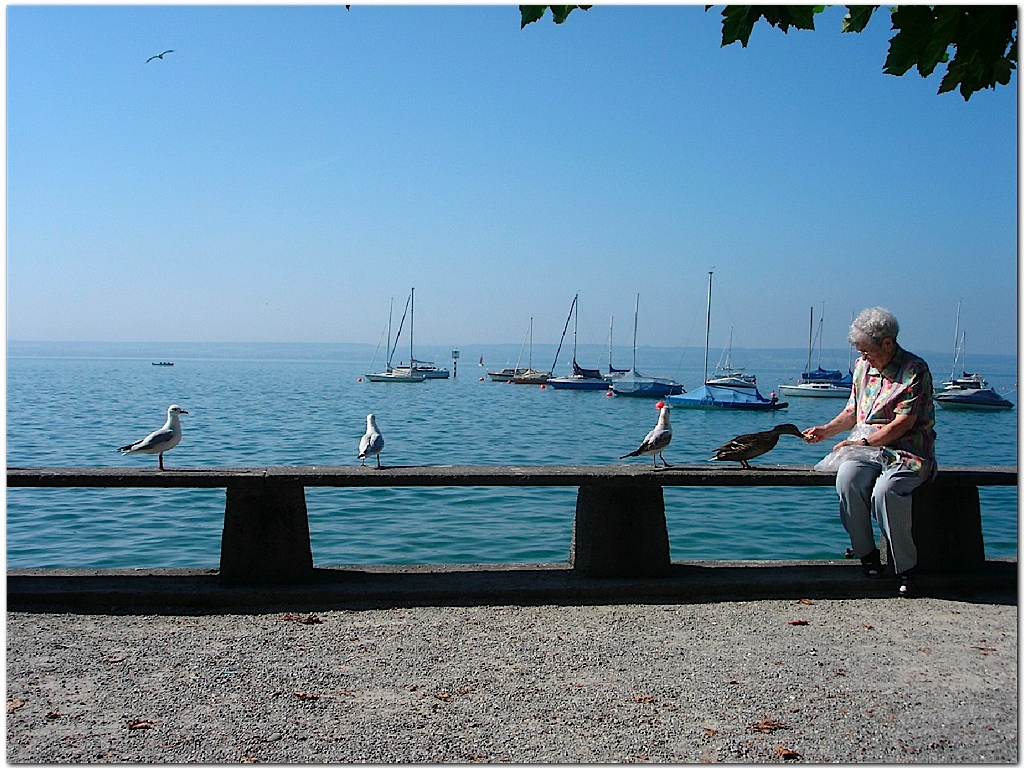
\includegraphics[width=300px]{images/DSC01957.JPG}\\
\textsc{Alimentando gaviotas y patos en el lago Constanza.} \end{center}

Avanc\'e 5~km y volv\'i a parar, mis piernas no quieren saber nada hoy. Da la
casualidad que era una playita, as\'i que --acord\'andome de que no me acuerdo
como es el Pac\'ifico-- me met\'i al lago, casi a la fuerza. Un poco sucio,
las piedras no dejan caminar (pero s\'i nadar), pero uno est\'a en Alemania
mirando a Austria en aguas de un gran lago sobrevolado tanto por aviones como
por dirigibles. \textquestiondown Vieron? De nuevo es la importancia de las
fronteras pol\'iticas: c\'omo uno siente diferente al acerc\'arseles. Es raro.

Pasando el mediod\'ia (\textexclamdown s\'olo 15~km en toda la ma\~nana!)
segu\'i viaje muy tranquilo, destino a Lindau si no pasaba nada. Y no pas\'o:
la ``Bodensee radweg'' est\'a muy bien marcada. Adem\'as est\'a llena de
turistas en bici, cosa que me encanta ver. Familias, parejas viejas y
j\'ovenes, amigos, todo el mundo viajando con las mochilas atr\'as y a pedal.
Ayer dorm\'i con un sueco que estaba haciendo un flor de viaje. Ahora
ven\'ia de Yugoslavia, Duvrovnik. Hoy segu\'ia por donde yo vengo, y se
babeaba en ``alemanglish'' con la ``Romantische Stra\ss e''.

Llegu\'e un poco temprano a esta maravilla de ciudad hist\'orica, las calles
son una preciosura; los edificios, una obra de arte. Ahora los miro desde el
faro al que acabo de subir, nunca v\'i uno tan lindo y adornado. Est\'a en la
punta de una escollera, que enfrenta a otra gobernada por un le\'on; recuerdan a
los lobos marinos marplatenses. D\'ia claro, un barco tur\'istico que cada media
hora entra y sale tocando sus bocinas, pocos turistas dandome vueltas alrededor
del faro, y dos regatas que salen del muelle. \textexclamdown Me encanta verlas!
Se mueven r'apido.

Com\'i banana ba\~nada en chocolate y una especie de caramelo pero que no es
caramelo. Delicia. \textexclamdown Qu\'e cambio de rumbo el m\'io, ehh! Por
fin los helados son un ``lujo'', ahora busco una buena relaci\'on
nutrici\'on/precio.

\textexclamdown Saludos alemanes hacia todo argentino que se les cruce!

Tute.

PD: Gustavo me espera (no sabe cu\'ando, como yo) con chivito al asador.
\textexclamdown Otra que el hijo pr\'odigo! \textexclamdown Ya lo veo a Felipe
quej\'andose! \textexclamdown Gracias, Gustav! Si va todo como lo planeo en
dos semanas llego a pedal a tu casa. Si me canso y tomo un tren, antes.
Adem\'as, tengo que pensar en el Sal\'on de Frankfurt. \textexclamdown Gracias
de nuevo!

\subsection*{Viernes 9 -- Immenstadt -- 60~km en 6:13 hs}

Aqu\'i se acaba de largar a llover, menos mal que ya estoy instalado.
\textexclamdown L\'astima que dej\'e toda el abrigo en donde me instal\'e!

Lindau estaba invadida de ara\~nas. \textexclamdown Llena de grandes telas
ocupadas por numerosas ara\~nas, en todos lados de la ciudad! Juro que ni pude
usar cabinas telef\'onicas, \textexclamdown incre\'ible! Nunca vi nada igual.

Hoy empec\'e con el bendito desayuno, acompa\~nado de una pareja alemana que
viajaba en bici por el lago. Lo sorprendente eran sus dos hijos, \textexclamdown
una de seis a\~nos! Charlamos un rato y me indicaron lo monta\~noso de mi ruta
para el d\'ia de la fecha. Como siempre, recib\'ia las noticias sonriente.

El clima amenazaba desde atr\'as, pero adelante el sol brillaba. La ruta, 508
creo, era con curvas seg\'un el mapa. Sub\'i a pedal unos 8~km (en vertical,
por poco necesito grampas y picos) por bosques. La cantidad de
curvas era imposible de dibujar en mi ahora poco detallado mapa. Desde arriba
ten\'ia una vista fenomenal, tom\'e muchas fotos. Cerros m\'as altos, mucho
bosque, casitas perdidas (buscaba caminos que las unieran pero nada, se
levantaban en medio del c\'esped), y abajo, el valle. Bajadas del 10\% seg\'un
carteles (que bajan 10 metros cada 100 recorridos) equival\'ian a 50~km/h sin
pedalear. Luego, suaves pero largas subidas; me desgastan m\'as que las de
mayor pendiente, porque intento hacer fuerza en lugar de entregarme a una baja
velocidad.

Par\'e en un banco de plaza mirando al valle. En algunos hosteles ofrecen
bidones de t\'e fr\'io, rojo y sin az\'ucar; tom\'e el que ten\'ia en la
botellita grande. Hab\'ia aviones por todo el cielo. Me sorprendi\'o el ver a
lo lejos mi misma ruta, que hac\'ia \emph{varios} minutos hab\'ia transitado.
Desde ahora har\'ia siempre eso: {\small V} cortas en c\'irculo, apuntando a
un mismo caser\'io (imaginen una pizza, lo cortado es el camino y el centro el
caser\'io). La sensaci\'on de no avanzar me cansaba, si bien el paisaje era
inmejorable. Menos mal pens\'e parar en Immenstadt porque estaba m\'as lejos
de lo pensado, aunque F\"ussen (destino inicial) estuviera a su vez m\'as
cerca de lo pensado: 60~km para el primero, 35 m\'as hasta F\"ussen. Imposibles
en el d\'ia de hoy.

Las altas y nerviosas monta\~nas suizas (antes lejanas) ahora serv\'ian de
fondo a las suaves, y ahora m\'as altas, sierras alemanas. \textexclamdown En
una bajada en recta llegu\'e a 74~km/h! En bici se siente m\'as la velocidad que
en cualquier veh\'iculo motorizado. Se la ve.

Luego de bordear un lago llegu\'e a Immenstadt a las 13:05. \textexclamdown Lo
not\'e porque de 13 a 14 cierran hasta los buzones en Alemania!
\textexclamdown No hab\'ia ni una \emph{B\"ackerei} abierta! Un super y una
fruter\'ia calmaron el hambr\'in. Esper\'e en una linda plaza central a que
abriera informaci\'on tur\'istica, y me indicaron una \emph{Gasthaus} donde
parar. \textexclamdown Cercana seg\'un los mapas, pero alta subiendo a la
monta\~na! Se nota la falta de aire en ese punto de la a\'un ciudad.
\textexclamdown Y se ve tan cerca!

Es la casa de una se\~nora de unos 70 a\~nos, m\'as simp\'atica que un perro
labrador; l\'astima que hablo poco alem\'an. Me di una ansiada ducha: en
subidas uno transpira densamente, y ni mis cejas de gallego pod\'ian
contenerla. Despu\'es sal\'i a recorrer la ciudad, momento en que empez\'o una
lluvia acompa\~nada de truenos. As\'i es que en una galer\'ia de una plaza
escribo mientras miro c\'omo la gente camina con paraguas (qu\'e envidia),
c\'omo se riegan las flores de los balcones, y escuchando las gotas (que
hac\'ia tempo no escuchaba, \textexclamdown espero no tener que hacerlo por
mucho tiempo!) sobre mi sombrilla.

Austria debe ser divino, en fotos desde Alemania con buena visibilidad se ven
sus picos nevados. Vi un cartel que indicaba una ciudad austriaca con marquita
``A'', a s\'olo 2~km. Lo segu\'i para pisar otro pa\'is pero un cartel de la
Uni'on Europea indic\'o, a la misma vez que cruzaba, que empezaba una autopista.
Volv\'i por mi camino con ganas de haber conocido.

Me espera ahora un panote de esos alemanes con semillas de cena, por s\'olo
\geneuronarrow{1}. \textexclamdown Parezco el vendedor de la panader\'ia!
Voy a ensanguchar una banana, y ma\~nana o pasado les contar\'e c\'omo estaba.

\subsection*{A partir del 10 de Septiembre -- El viaje desde Immenstadt}

\emph{Pas\'e varios d\'ias sin escribir mails, pero los le\'ia. Continuaba,
eso s\'i, escribiendo en mi maltrecho cuaderno. Antes de transcribirlo envi\'e
este resumen a un hermano, en que contaba c\'omo continu\'o el viaje, y c\'omo
regres\'e a G\"ottingen.}\\

\textexclamdown Hola Rami! Gracias por tu mail. Te escribo en breves l\'ineas
lo que sigue al diez: llegu\'e a F\"ussen y conoc\'i los grandes castillos, un
buen lago, monta\~nas altas, divinura. Hice la mitad del viaje tras un
ciclista alem\'an m\'as bueno que el pan lactal. Despu\'es segu\'i viaje por
la \emph{Romantische Stra\ss e}, \textexclamdown 100km! Cuando llegu\'e a
Landsberg y tuve problemas con hoteles llenos (s\'i, un poco por falta de
plata, pero fue m\'as bien una excusa) tom\'e un tren a Dachau
(\emph{Dajau}), ya que no sab\'ia como unirlo en bici del mejor modo, un
desv\'io de 50~km, ``\emph{not big deal}'' para el proyecto de circuito a
pedal.

Dorm\'i all\'a y conoc\'i el campo de concentraci\'on nazi, que luego de ver
libros lo \'unico nuevo fue la piel de gallina de estar pisando el mismo suelo
y respirando el mismo aire (al oler la madera de las literas me inquiet\'e
mucho, pero son reconstruidas) y pasando a trav\'es de la misma puerta
``\emph{arbeit macht frei}'' (``el trabajo los har\'a libres''), que para los
creyentes fue verdad: hijos de puta. Lo que s\'i me movi\'o diferente de lo
que ya conoc\'ia fueron los crematorios, ``\emph{dead chambers}'' (almac\'en
previo al crematorio) y c\'amaras de gas (me sorprend\'i en una sin saberlo y
el chorro de adrenalina fue suficiente como para necesitar acercarme a una
persona y sentirme un poco a salvo de la historia). Y me dej\'o pensando en
c\'omo un nazi, por m\'as fanatismo que tenga, puede creer que est\'a haciendo
bien, puede quererse creando tanto mal, y suponiendo que s\'olo fuera una
persona. Justamente tal vez por la cantidad y falta de personalidad uno puede
creer, como el nazismo pretend\'ia, que \'esas no son personas.

Un folleto de la historia de la ciudad, que empieza desde el 800dC, dice que
tristemente ahora el nombre Dachau no se asocia a la ciudad de artistas y
comercio en la ruta Augsburg-M\"unchen que era antes. Es verdad: lo dijo la
expresi\'on de la de informaci\'on tur\'istica al yo preguntarle; lo dice el
folleto; lo dijo un jud\'io sobreviviente (frase en la entrada del campo); lo
mostr\'e yo al preguntar por eso antes que por el castillo.

En el tren a Dachau pensaba ``qu\'e lindo que me lleve a G\"ottingen'' y as\'i
me di cuenta de que extra\~naba por lo que, luego de conocer all\'a:
\textexclamdown tren a casa! Y ac\'a escribo, desde mi {\small PC} y sin
Romantische Stra\ss e, y sorprendentemente para m\'i (a pesar de no haber
completado el viaje planeado) {\small CONTENTO}.

Me cans\'e de estar solo, es la raz\'on principal y verdadera. Traste y
piernas son un viol\'in, seguir\'e saliendo a correr seguramente. Me esperan
todav\'ia el sal\'on del autom\'ovil, el museo en Wolfsburg, y dem\'as cositas
``kinder'' que se ir\'an presentando.

Ese es el resumen, \textexclamdown ya mandar\'e el detalle! \textexclamdown No
se librar\'an de mi!

\textexclamdown Gracias por \emph{todos} sus mails! No saben qu\'e alegre los
leo y c\'omo me sirvieron durante el feliz pedaleo.

PD: La noche de ayer que estaba de fiesta por volver a casa despu\'es del
\emph{Viaje} tom\'e mi primer cerveza sin que me ofrezcan. Hace tres meses que
no tomo nada, y tomar vac\'io mientras esperaba el plato bast\'o para que mis
pasos (m\'as 100~km recorridos, y esta debe ser la verdadera raz\'on) ya no
sean tan precisos.

\subsection*{S\'abado 10 -- Immenstadt -- 0~km}

Hoy me levant\'e y llov\'ia, desde ayer sin parar. Encontr\'e poco por hacer,
casi que dependo de la bici. Claro, estar al pedo solo no es lo mismo que
acompa\~nado. Luego del suficiente desayuno sal\'i a caminar bajo la lluvia.
Recorr\'i, mand\'e cosas a casa por correo, compr\'e ``El amor en tiempos de
c\'olera'' (incre\'ible como escribe Gabriel Garc\'ia M\'arquez: hace una
prosa poetizada, con tantas palabras que m\'as de una vez necesito
diccionario), y tambi\'en un s\'andwich para almorzar.

Una ducha por el fr\'io; le\'i hasta que el ruido de la lluvia, tan
rom\'antico ayer a la tarde, me desesper\'o. Sal\'i de nuevo a caminar,
Immenstadt es una bonita ciudad. Me sent\'e en una galer\'ia de la plaza
central, y se ve\'ian los cerros al fondo siendo tragados por las nubes.
Camin\'e hasta la entrada del pueblo, se ve\'ia ahora la niebla
levant\'andose. \textexclamdown Se iban las nubes! Lo gris se mov\'ia, entraba
luz y dejaba de llover.

Pas\'e la \emph{Gasthaus} y sub\'i hasta la m\'inima capilla que se ve desde
mi ventana, divina vista tiene. Simpleza total. Donde ir\'ia el altar hay
im\'agenes que recrean a la crucifixi\'on. Cinco bancos de iglesia a cada
lado, y el v\'ia crucis externo, que parece una sucesi\'on de l\'apidas
rodeando la capilla. Un fresco en el alto techo era el \'ultimo detalle.
\textexclamdown Simple y hermosa!

Sub\'i a mi habitaci\'on y mir\'e por la ventana, vi al cielo ya no
homog\'eneamente gris, sino con las infinitas tonalidades de las numerosas
nubes tocadas por el sol, que se esconde.

Baj\'e a cenar luego de lecturas a las ``\emph{halb acht}'' (7:30 no 8:30,
menos mal que tengo apuntes). Ah\'i, siete amigos que promediaban los
cincuenta tomaban, com\'ian y re\'ian. Ninguno hablaba otro idioma adem\'as
del alem\'an, as\'i que les devolv\'i agradecido el ``\emph{Guten Apetit}''.
Por se\~nas (muy f\'aciles de imaginar) les pregunt\'e si eran ellos los que
anoche guitarreaban. Se escuchaba m\'usica t\'ipica alemana, pero cre\'i que
ven\'ia de la casa de al lado. S\'i, eran ellos, as\'i que me invit\'e a
unirme esa noche. ``\emph{Sehr Gut!}'', contestaron. Apenas empec\'e a cenar
me dejaron su Leberwurst, riqu\'isimo. Cuando termin\'e el pan fui a buscar
m\'as y notaron que no encontraba, as\'i que me dejaron el de ellos. No
contentos con eso me dejaron una salchicha ahumada, riqu\'isima. Tambi\'en me
ofrecieron Brandy (\'unica bebida alcoh\'olica aparte de la cantidad de vino y
cerveza) que a pesar de mi curiosidad por conocer negu\'e.

Sub\'i hasta que empezaran a guitarrear. Y vi el cielo libre de nubes, me
alegr\'o. Cuando baj\'e (con el diccionario alem\'an-espa\~nol) me ofrec\'ian
cerveza pero ya me daba verg\"uenza, as\'i que negu\'e hasta que insistieran.
Claro que no lo hicieron, \textexclamdown Murphy la ten\'ia clara al dictar
sus leyes! Estuvo buen\'isimo: una o dos horas de siete amigos alemanes
ebrios, cantando a coro y con dos guitarras su m\'usica tradicional. Me
preguntaron (con adem\'an de prestarme) si tocaba la guitarra. \textexclamdown
Me qued\'e con buenas ganas de cantarles ``El corralero'', \'unica que se y
por noches similares! Me animo a cantar por descarado, \textexclamdown pero de
la guitarra m\'as vale mantenerme alejado! Me contaban que esa tarde caminaron
hasta la cima de no-se-qu\'e-cerro, que no era gran cosa sino era por la
lluvia, el barro y la niebla. Son gente de un pueblo a 100~km de Karlsruhe,
turistas por el fin de semana, y cantan por hobby. La que m\'as me gust\'o
fue ``\emph{Kapitano}''. Me sorprendi\'o su inter\'es en que nos
entendi\'eramos. \textexclamdown Igual creo que me perd\'i diecisiete chistes!

\textexclamdown Como a las 10 pm nos dio sue\~no! La guitarreada empez\'o a
las 8 pm, gran diferencia en las costumbres con nuestras pampas. Nos acostamos
luego de mirar el claro cielo con poco de niebla. Cama c\'omoda como pocas
veces, la disfrutar\'ia hasta las 8 am, hora en que nos despertar\'ian.
\textexclamdown A disfrutar de la ma\~nana en Alemania! Y c\'omo lo har\'ia
esta.

\subsection*{Domingo 11 -- F\"ussen -- 50~km en 2:15 hs}

Hoy me levant\'e a las 8 am, no se ve\'ia un chosno. La niebla ni siquiera
dejaba ver el color del cielo, y estaba un poco fresco. Sal\'i igual a pedalear
luego del desayuno: los pron\'osticos indicaban lluvia para la tarde y no le
erran. Suelo h\'umedo pero no mojado; en la noche no hubo chaparrones.

Apenas sal\'i de los l\'imites de Immenstadt\ldots\ \textexclamdown
desapareci\'o la bruma! Mir\'e atr\'as y la ciudad estaba inundaba por densas
nubes, muy sorprendente. Ve\'ia niebla arriba en los cerros o en mi ex-ciudad,
pero no en mi camino, cosa que me alegr\'o por poder ver los siempre enormes
paisajes. Los caracoles de subida que anunciaban mi mapa no fueron tan
interesantes (o me equivoqu\'e de ruta), pero todo el camino presum\'ia de
belleza en cada kil\'ometro.

Me pas\'o un ciclista rutero, y creo que me pregunt\'o si iba a F\"ussen. Le
dije que s\'i: si preguntaba si ese era el camino la respuesta era igual. Nos
cruzamos otra vez, otra y despu\'es otra. En las bajadas yo pedaleaba as\'i
que me acercaba, \textexclamdown pero \'el sub\'ia como si viajara en bici!
Entonces desaparec\'ia. En la tercera vez que lo encontr\'e, parado
sac\'andose abrigos de las piernas, fren\'e y empezamos a charlar. No se
porqu\'e me dijo que casi no hablaba ingl\'es: vivi\'o un a\~no en Orlando
Florida trabajando para ``\emph{Universal Studios}'', donde ve\'ia a diario la
r\'eplica del gran castillo que estaba yo por visitar: \emph{Newschwanstein}.
De Essen el hombre, se sorprendi\'o de que la mochila fuera todo mi equipaje.
Yo me enorgullec\'i de eso, y le cont\'e mi viaje. Nos sacamos foto en un lago
(parezco el turista japon\'es) y seguimos viaje. Me llev\'o como lech\'on pal'
pueblo, pero como cortaba el viento se sinti\'o poco. As\'i que llegu\'e al
mediod\'ia y con traste nuevo, despu\'es del descanso de ayer y pocas horas de
hoy. Al entrar al pueblo lo desped\'i pero lo cruc\'e dos veces m\'as: al
salir de las oficinas (\'el entraba), y al subir a los castillos m\'as tarde
(\'el bajaba).

Qu\'e diferencia: \textexclamdown hoy no me alcanz\'o el tiempo! Dej\'e bolsos
y sal\'i en la bici al centro tur\'istico. Calles estrechas y zigzagueantes,
casitas antiguas con carteles de metal sobresaliendo, galer\'ias con no
demasiada gente\ldots\ en una cuadra hab\'ia varias casitas muy similares,
pero de colores tan distintos que parec\'ia un dibujo de primaria. Almorc\'e
una bomba de panader\'ia inc\'omoda (ten\'ia forma de bomba, literalmente)
sentado en una fuente, y mirando y escuchando a un trompetista. Al encarar
hacia los castillos escuch\'e una gran banda. Me acerqu\'e y era estilo
militar, con muchos instrumentos de viento y director al frente. Las bandas
numerosas me emocionan, la observ\'e hasta que me picaron las hormigas (que no
despert\'e a prop\'osito).

Me separaban 5~km hasta los castillos. Me sorprendi\'o la ciclov\'ia, por su
cartel de ``\emph{Romantische Stra\ss e}'', ruta que seguir\'ia con \'unico desv\'io
hacia Dachau. \textexclamdown Los folletos muestran 20 pueblos con detalles
interesantes por conocer en esas decenas de kil\'ometros de calle rom\'antica!

Cuando divis\'e el castillo grande y m\'as nuevo sent\'i lo mismo que al
encontrar el lago Constanza: un punto de referencia grande en los planes del
viaje. Emocionad\'isimo sub\'i hasta encontrar el ``\emph{Ticket center}''. No
se r\'ian del viajero, pero juro que se parec\'ia a un aeropuerto. Lleno de
gente, una cola larga hasta las 4 ventanillas de venta, y monitores indicando
las ``pr\'oximas salidas''. ``Salgo a la hora que quiero'' pensaba yo, hasta
que el vendedor me pregunt\'o:

\subparagraph{}\label{ssub:hayGuia} --- \textquestiondown Gu\'ia en
ingl\'es?\\ --- No, gracias. Voy por mi cuenta.\\ \hangindent=1cm

Pero resulta que no est\'a permitido, as\'i que me citaron a las 13:15 en
\emph{Hogenschwangau} --menos mal que fue el primero-- y a las 15:25 en
\emph{Newschwanstein} --menos mal que fue el segundo.

Lo primero que encontr\'e camino al primero fue un hermos\'isimo lago rodeado
de monta\~nas bajas y boscosas. Las monta\~nas m\'as altas todav\'ia tienen
nubes atascadas, \textexclamdown que no se pinchen y se largue a llover!

Encontr\'e todo incre\'iblemente lujoso (como es de esperarse en un castillo,
creo), adem\'as de lindo. Lleno de condecoraciones, le pregunt\'e al gu\'ia si
la familia real iba a la guerra. ``Algunos mostraban su valent\'ia'', fue toda
su explicaci\'on. Dise\~no a la antigua, con almenas (esos ladrillos cuadrados
en los que uno imagina escondido detr\'as a un arquero); y color a la
vanguardia: anaranjado y amarillo. Vista que asombra. Tras una ventana hab\'ia
algo similar a un telescopio, pero en vez de apuntando al cielo, apuntaba a lo
que eran entonces las construcciones del nuevo castillo de Ludwig II:
\emph{Newschwanstein}. Luchito para los amigos --o luch\'in, porque me qued\'e
con dudas sobre su preferencia sexual seg\'un charlas de la gu\'ia-- segu\'ia
las construcciones de su nueva casa desde su casita anterior. \textexclamdown
Locura Real! Para visitar al ``vecino'' se baja una monta\~na y se sube a la
otra.

Baj\'e a ``\emph{ticket center}'' para subir al otro castillo por donde lo
hacen los colectivos, que es m\'as largo y en curvas que el camino peatonal.
Es una ``{\small V}'' corta que sube a la monta\~na, de sentido \'unico y no
mucho lugar para maniobrar, con sem\'aforos en la salida y la llegada.
Esper\'e bastante al verde del sem\'aforo abajo, hasta que me pas\'o un
colectivo (usan controles remotos para cambiar las luces) y pedale\'e
tranquilamente pero sin parar, viendo cada vez m\'as el lago Alpsee. Al llegar
a la curva empezaba a caer una fina lluvia, que el bosque mantuvo en sus hojas
hasta que llegu\'e al techo de la parada de colectivos, cercana al
``\emph{Marienbr\"ucke}''. ``\textexclamdown Pararse en ese puente justifica
un viaje a Europa, Tu!'', ya hab\'ia advertido mi t\'io. Dej\'e la bici
ah\'i y sub\'i al puente para corroborarlo.

Se siente hermoso tan solo describirlo. Lo construy\'o primero un
rey para disfrutar de la vista al valle. Abajo corre un curso de agua, y
justito abajo en vertical hay una olla donde desemboca una
cascadita, que si no fuera por los 34 metros de altura dan ganas de tirarse.
Luego Ludwig embelleci\'o el puente para ver, aparte del paisajazo y lagos
\emph{ForggenSee} y \emph{BunnwaldSee}, a su nuevo ejemplo de excelent\'isima
arquitectura, el castillo que ahora visitar\'ia. El mal clima permiti\'o una
particular vista. Sin taparme las monta\~nas y lagos (los hac\'ia parecer
m\'as lejanos), las nubes se apoyaban sobre los picos m\'as altos.
Bell\'isimo. \textexclamdown Con sol se debe ver hasta el Mar del Norte!

Luego esper\'e 20 minutos en la entrada del castillo bajo la lluvia, rodeado
por los blancos muros, las monta\~nas y la ca\'ida de agua. Ya en la visita,
me impresion\'e con las dos millones de partes que componen el brillante
mosaico del suelo de una sala, con la apertura al p\'ublico por parte del
estado s\'olo seis semanas luego de la muerte del sin herederos Ludwig II, y
con su habitaci\'on que merece p\'arrafo aparte. Y todo esto, sin contar que
no lograron terminar la obra antes de su muerte, y de hecho actualmente hay
habitaciones vac\'ias.

Su habitaci\'on da a la cascada, as\'i que siempre hay ruido a la fuente de
vida (el libro de la n\'omada del desierto africano me conmovi\'o, como
notar\'an). Hubiese descripto el estilo como similar a la catedral de
Estrasburgo pero gracias a que me enchufaron gu\'ia ahora s\'e que es
``g\'otico''. La cama parece en s\'i misma una catedral, con el techo inundado
de ornamentos en madera. No me salen las palabras para describirlo, y cuando
estudi\'e G\'otico seguro las memoric\'e. Las paredes y columnas (todo de madera
oscura) tienen un trabajo de precisi\'on incre\'ible: \textexclamdown 4 a\~nos
de trabajo llev'o esta sala! La puerta se camufla entre los adornos del estilo y
me encant\'o la gran cerradura y picaporte. Su sill\'on de lectura lo tall\'o un
duende, no un humano porque sus manos ser\'ian demasiado grandes y menos
precisas. Me sorprendi\'o su capilla propia, de 2$\times$2 m, con lugar para el
Sant\'isimo y todo. Los reyes ten'ian l'inea directa parece.

En las pinturas de guerra (cientos de guerreros a pie o caballo clav\'andose
lanzazos) no se ve sangre por ser considerada ``anti-est\'etica''.
\textquestiondown Y desde qu\'e aspecto la guerra lo es? S\'olo, al menos y
mir\'andola con demasiado cari\~no, el esp\'iritu de entrega absoluta por una
causa que algunos creen justa. Pero es eso justamente lo que evitaron mostrar
en las grandes pinturas del enorme comedor. Sobre tama\~no de cocinas, \'esta
aproximadamente ocupa una hect\'area. Hab\'ia una mucho m\'as chica para la
servidumbre seguro, aunque me sorprendi\'o no usaran la misma.

En los mapas de la zona no se ven cercanos los lagos al castillo, por eso no
entend\'ia las postales con todo juntito. Es que los castillos est\'an altos
en la monta\~na; desde all\'i se ve el lago perfectamente, y la ruta
rom\'antica saliendo hacia el Norte. Aunque en realidad no est\'an en la punta
de un cerro, como en las suaves colinas del centro de Alemania: el precipicio y
las rocas de aqu\'i imposibilitar\'ian la construcci\'on.

A la salida camin\'e hasta mi bici y me abrigu\'e para evitar mojar mi ropa en
la bajada, hab\'ia dejado de llover. Guard\'e el cuaderno en una bolsa junto
con un vaso alem\'an nuevo (\textexclamdown por fin uno que me encanta!), y
at'e el candado atr\'as porque se caer\'ia si lo dejaba sujeto al cuadro.
Luego de pedirle a un chofer que me diera luz verde, me tir\'e. Mientras,
quienes esperaban al siguiente colectivo me miraban, \textexclamdown no se si
envidiosos, o como a un loco!

No anduve muy r\'apido, era peligroso en bajada y con agua, entre el humilde
ancho del camino y el precipicio. Hasta donde los nervios me permit\'ian.
Usaba los dos frenos pero, acostumbrado al peso de las mochilas, us\'e
demasiado el trasero y en una curva di una derrapada, que no por exagerada
como por la velocidad y condiciones del camino, es que me dio El Susto.
Siempre me siento controlado en dos ruedas, pero sobre agua nunca: me di
varios y sorpresivos golpes por no medir bien los l\'imites. Siempre recuerdo
con cari\~no uno yendo a la escuela, porque era invierno y estaba todo abrigado,
as\'i que s\'olo se escuch\'o la campera, la mochila y los pedales raspando
contra la calle. Cuando no pasa nada malo es divertido pero ac\'a no pod\'ia
asegurar la misma suerte. Por suerte (seamos sinceros, \textexclamdown por
perfecto dominio!) la cola de la bici volvi\'o a su lugar y continu\'e la
bajada, hasta el primer techo que encontr\'e en el punto comercial.

Foto a la cara de felicidad despu\'es de la adrenalina, \textexclamdown y a la
caliente ducha del hostel, sin paradas! Si ma\~nana llueve, envuelvo el equipaje
en bolsas y sigo vestido como hoy, seco y calentito.

Volv\'i por una gran plaza y de nuevo las encontr\'e sorprendido: bolsitas de
basura en un dispenser para recoger los restos de los cachorrines, y mantener
as\'i el pasto y caminos limpitos. Otro comentario: vi varias veces caballos
de equitaci\'on y ni\~nos entrenando, no saben lo bellos que son. A los
caballos no les cortan los crines ni la cola, son de color chocolate,
musculosos y de todos los tama\~nos. El ni\~no, o ni\~na m\'as generalmente,
con botas largas de cuero, pantal\'on blanco o negro, camisita blanca y
casquito negro, sentados derechos sobre el animal que camina con buena
presencia. Me encantan. Tambi\'en cruc\'e dos personas en bici con demasiados
bolsos y entonces me fij\'e en su banderita: ``la vuelta al mundo''.
\textexclamdown Que l\'astima \'ibamos en sentido contrario y no pude charlar!
El sue\~no del pibe.

Llegado a la ducha, mi cara cambi\'o\ldots\ \textexclamdown y no para bien! Esta
ducha es como otra que ya tuve: una incre\'ible presi\'on, y el agua tan
pulverizada que de verdad arde. Panza y cabezas, resguarecidas.
\textquestiondown Pueden creer que una ducha haga mal? \textexclamdown Es como
comer un poco de pan de salvado y caiga pesado! Y uno entra con esperanzas de
salir renovado, relajado, descansado; y sale todo maltrecho como si viniera de
un viaje en bici bajo lluvia. \textexclamdown Incre\'ible! Y ya lo mencion\'e,
\textexclamdown las nuevas experiencias que tengo en Alemania son dif'iciles de
olvidar!

\subsection*{Lunes 12 -- Dachau con trampita -- 100~km en 5:32 hs.}

Hoy fue un buen d\'ia largo. Empez\'o temprano con un desayuno en una luminosa
galer\'ia, con buena vista a un parque. Despu\'es de pasear un poco por las
cercan\'ias de F\"ussen hasta por fin encontrar la Romantische Stra\ss e para
bicis, la segu\'i. Es comod\'isima, bien se\~nalizada y lejos de los autos.
Paisajes incre\'ibles, una niebla levant\'andose, y el gran castillo de fondo
por largo tiempo acompa\~nando, rodeado de cerros y de bosques. Clima bastante
fresco y cielo de todos los colores: pod\'ia salir el sol como venir un
tornado. Se decidi\'o por lo que los pron\'osticos predec\'ian: nublado sin
siquiera llovizna.

Conoc\'i \emph{Wieskirche}, una iglesia con m\'as fama que Chatr\'an.
Entr\'e pensando ``porqu\'e tanto espamento'' y entonces entend\'i. En vez de
ser con forma de cruz y techo de la misma altura, en el medio se levanta una
b\'oveda como joroba, que del lado interno presenta frescos; todo bello,
lujoso, y viejo pero preservado perfectamente. Saqu\'e la foto a una firma
grabada en uno de los ornamentales bancos de madera del a\~no 1800, mi t\'io
informa que las hay mucho m\'as viejas. Me impresionan siempre los \'organos y
el lugarcito desde donde el sacerdote dar\'ia la homil\'ia, un piso m\'as
arriba sobre un costado de la nave central. Siempre con incontables adornos.

No me cans\'e de sacarle fotos al paisaje y tambi\'en al cielo, siempre
cambiante. Este cielo les har\'ia creer que soy buen fot\'ografo y todo.
\textquestiondown Vieron los cielos que uno ve pintado en acuarelas, o que se ve
en un campo e inspira ganas de pintarlo? Bueno, ac\'a est\'a todos los d\'ias,
uno lo puede ver mal por falta de sol o bello por los infinitos colores que lo
decoran. Las formas de las nubes, las avionetas apareciendo y
desapareciendo\ldots\ \textexclamdown Interesante mientras no llueve!

Al salir de \emph{Wieskirche} hay una capillita de las que a mi me gustan, de
5m$^2$, con figuras de la crucifixi\'on y un fresco de Jes\'us atado durante
los azotes, todo ensangrentado, que no dej\'o de impresionarme. Encorvado y
sufriente. Para colgar cerca de los cuadros de guerra de \emph{Newschwanstein}
estaba. Cre\'i que esas im\'agenes s\'olo se ve\'ian en la pel\'icula ``La
Pasi\'on'' pero vean, en esta capilla que ni siquiera a ello llega, hay un
cuadro vaya uno a saber de qu\'e a\~no. Hace pensar, por la crudeza, en lo que
uno piensa luego de ver esa pel\'icula.

Esta ciclov\'ia rom\'antica pasa por lo lindo de las ciudades lindas, con lo
cual los 100~km no se permitieron un segundo de aburrimiento o gran cansancio.
En un pueblucho cualquiera, en una fuente cualquiera de una plaza cualquiera,
hay una estatua de bronce de un gordito pelado, sonriente, con los pies bajo
el agua y la mano tocando la superficie, como probando la temperatura. Sus
chancletas esperan al lado de la fuente. \textexclamdown Todo est\'a adornado!
Vi lo que la vieja me describ\'ia antes de mi viaje, pero cerca de G\"ottingen
en realidad: las dobles ventanas con adornos en el medio, cortinas desde la
mitad para abajo, detalles que hacen de una casa un hogar pero que no las ve
s\'olo la familia sino cada transe\'unte. Entr\'e en una iglesia de otro de
estos pueblos y justo ensayaban con el \'organo. Otro aderezo m\'as, esta vez
para oir.

Luego, y cuando promet\'i no parar m\'as para poder llegar a Landsberg, par\'e
para ver a un avi\'on que sub\'ia y bajaba, y sub\'ia y bajaba, todo el
tiempo, y cambiaba de altura bastante r\'apido. Tiraba paracaidistas
descubr\'i luego, siempre de a tres que se dejaban en ca\'ida libre por un
rato y luego los abr\'ian. El avi\'on se perd\'ia constantemente entre las nubes
bajas, a los aventureros les debe haber hecho m\'as picante la experiencia.
Entonces promet\'i no parar m\'as, y a la vuelta de la curva hab\'ia, armada con
le\~nos que por ac\'a abundan, la forma de la fachada de una casa. En vez de
mantenerlos embolsados para guardarlos les dieron una forma m\'as particular y,
claro, bella. Par\'e para sacar foto mientras la molestia de no cumplir con el
plan se mezclaba con la alegr\'ia de no poder dejar de sorprenderme.

Luego segu\'i los 30~km hasta Landsberg, pensando en c\'omo unir Dachau, y
cuantas noches usar en ``desviarme'' hacia el Este de lo conocido (al menos por
mis folletos). Me interrumpi\'o los pensamientos un avi\'on grande, parec\'ia
los que usan los bomberos para los fuegos en bosques pero de colores militares.
Enorme y a muy baja altura, segu\'ia el curso del r\'io que yo bordeaba.

Llegu\'e a la ciudad y me fascin\'e con su centro tur\'istico. En
informaci\'on me indicaron que todo estaba lleno, me mandaron a la estaci\'on
de trenes que quedaba cerca, pero ah\'i me dijeron que no hay habitaciones. Un
hombre vio que necesitaba ayuda, y muy amablemente me acompa\~n\'o media
cuadra hasta una pensi\'on que ofrec\'ia n\'umeros telef\'onicos a falta de
recepcionista. Al mostrarle mi falta de tel\'efono fue a buscar el de su casa,
pero no atend\'ian. Lo vi tan hospitalario que le ped\'i indirectamente un
suelo para echar mi bolsa de dormir, pero me contest\'o evasivamente, aunque
de buen modo, que no sab\'ia quien pod\'ia prestarme un suelo.

S\'olo quedaba un hotel a \geneuronarrow{55}, la temporada alta se hace
sentir. A rega\~nadientes acept\'e, pero cuando sub\'i y vi que la
habitaci\'on era fea y oscura, hice unos llamados para solucionar unas cositas
todav\'ia de la tarjeta y ped\'i el checkout. \geneuronarrow{30} de llamadas
(\textexclamdown terrible!) y verificaron que no me haya ba\~nado. Todo estaba
bien: limpi\'e el inodoro que ven\'ia necesitando desde hac\'ia kil'ometros. No
me importaba si ten\'ia que no dormir, o dormir sentado en el centro
tur\'istico, pero no dejar\'ia la plata de dos o hasta tres noches en un lugar
que no me gustara. Mientras empacaba la bici pens\'e en tomarme un tren a
Dachau: solucionaba el ``problema'' de c\'omo unirlo, dormir\'ia bien
(r\'apida y astutamente descart\'e la opci\'on de prescindir de cama) y al
otro d\'ia seguir\'ia la ruta planeada.

Y as\'i fue, para completar los 50~km que restaban a Dachau tuve que tomar
tres trenes (me estoy poniendo canchero con el manejo en tren por Alemania)
pero fue barato y no muy inc\'omodo. El problema es que al subir corriendo al
pr\'oximo tren empezaba a pensar: ``\textquestiondown no me habr\'e olvidado
algo en el anterior?'' \textexclamdown Ninguna respuesta servir\'ia en este
nuevo tren! De todos modos y por suerte siempre eran respuestas negativas.

En el tren pensaba: ``qu\'e hermoso que este tren me lleve a G\"ottingen''. Y
entend\'i entonces que estaba extra\~nando, y tal vez por eso quer\'ia hacer
100~km y no parar en ciudades lindas como Landsberg, tal vez por eso estaba
gru\~n\'on. Tambi\'en me ten\'ia inc\'omodo que ya me quedaba de nuevo sin
plata, pero esa era la excusa. Decid\'i conocer Dachau y al d\'ia siguiente
tomarme un tren a casa; los 15 minutos de viaje que todav\'ia faltaban fueron
euf\'oricos. \textexclamdown Qu\'e alegr\'ia! \textquestiondown Porqu\'e, si
no hago lo que quer\'ia? Porque hice {\sl mucho m\'as} de lo que quer\'ia, y
ma\~nana voy a volver a estar c\'omodo y sin extra\~nar. Como en casa,
despu\'es agradec\'i a Gustavo que pudiera sentir esto en Alemania. As\'i,
cada vez m\'as contento, llegu\'e a Dachau.

Baj\'e del tren y segu\'i al mal\'on, que se iba r\'apido como si vivieran en
Buenos Aires. Era para el otro lado del centro y me di cuenta por la falta de
luces, sin embargo me sorprendi\'o, pues supuse que la mayor\'ia encarar\'ia
para all\'a, donde necesito. Le pregunt\'e a un chico que jugaba al basket y me
mand\'o al lejano hostal, que no fue dif\'icil de encontrar.

\textexclamdown Hostal canchero y moderno como pocos! Y con el precio de
hostal juvenil. L\'astima que no ten\'ian lugar. Puta suerte, ya eran las 21 y
estaba estrenando las luces de la bici, quer\'ia llegar a alg\'un lugar e
instalarme. El recepcionista, un no-joven muy servicial, me indic\'o una
\emph{Gasthaus}.

\subparagraph{}\label{ssub:hostalLleno} --- Un minuto, llamemos antes para ver
si tambi\'en est\'a llena -- contest\'e.\\ --- Bueno, \textexclamdown ah\'i
ten\'es un p\'ublico!\\ \hangindent=1cm

No esperaba esa respuesta, pero ten\'ia la tarjeta telef\'onica con que
llamaba a Gustavo. La nueva casa ten\'ia lugar, y lo reserv\'e con gusto.

Tambi\'en fue f\'acil llegar, todo por avenidas, siempre tomando la
bifurcaci\'on izquierda. Estaba al lado de Informaci\'on Tur\'istica y del
castillo, pleno centro y barat\'isimo por ser \emph{Gasthaus}. Cuando me
dieron las llaves de la habitaci\'on n\'umero 1 sent\'i endorfinas por todo el
cuerpo, \textexclamdown por fin! M\'as de 12 horas de viaje de puerta a
puerta. Guard\'e la bici lo m\'as relajado que pude, y al entrar pensaba que
por el doble de ese precio estar\'ia durmiendo ahora en un lugar feo y
planeando c\'omo llegar a Dachau, al otro d\'ia, en bici. Imposible de
pedalearlo, adem\'as, luego de los 100~km de hoy. Fue una buena decisi\'on.

As\'i que me relaj\'e, com\'i una gran ensalada con pollo (\textexclamdown
tuve que gastar de todos modos aquel no malgastado dinero!) y tom\'e la primer
cerveza de mi vida sin que me ofrezcan. Mitad mientras esperaba el plato,
mitad durante la sabros\'isima cena, as\'i que, y luego de pedalear 5 horas
(la verdadera raz\'on), ya los pasos no ser\'ian tan precisos. El lugar era
precioso, todo de madera, con doble ventana a falta de doble vidrio, vasos
alemanes sobre las alacenas, pinturas con im\'agenes t\'ipicas del lugar, diez
grifos rodeando la barra para cada tipo de cerveza\ldots\ un sue\~no t\'ipico.
Lo bueno es que mientras cenaba sonre\'ia solo, estaba empezando a asimilar y
pensar en todo lo que hice, en vez de planear qu\'e me esperar\'ia ma\~nana,
por primera vez en semanas. Ya estaba, \textexclamdown gracias por
acompa\~narme, piernas! Y todos esos pensamientos est\'upidos luego de cumplir
euf\'orico con algo propuesto. Mor\'ia por contarle a alguien pero no ten\'ia
el tel\'efono habilitado en mi habitaci\'on, menos mal porque me terminaba de
secar, sino. Y salir de mi hogar por fin encontrado por un tel\'efono, ni
ebrio.

Quise pagar con monedas pero no llegaba, as\'i que pagu\'e con el \'ultimo
gran billete. Los guachos notaron mis intenciones y el vuelto fue todo en
monedas, la mochila pes\'o un 20\% m\'as desde esa cena. Ba\~no de inmersi\'on
(con ese ocioso chorro, media hora esperando a que se llene la tina) y me puse
la tercer muda de ropa que no hab\'ia usado en todo el viaje, y su \'unico
olor era el del chocolate derramado cerca de Hann M\"unden, el primer d\'ia de
viaje. Vida nueva, una gran alegr\'ia. La mochila tuvo nuevo lugar
porque us\'e tambi\'en el jean poco engrasado y el buzo polar amarillo por el
fr\'io, que ocupa m\'as lugar que una almohada.

As\'i que dorm\'i perfectamente en una c\'omoda cama. Y ma\~nana al castillo,
info tur\'istica, y el campo de concentraci\'on de la II~Guerra Mundial para
terminar en la estaci\'on de tren. Todav\'ia no me imagino c\'omo ser\'a pero
de todos modos pienso poco, ya lo ver\'e.

\textexclamdown Qu\'e Lunes tuve! Otra que rutinario. Siempre me gusta pensar:
``hoy me levant\'e en F\"ussen'', y no puedo creer que todo haya sido en un
solito d\'ia. Pensar que el tiempo siempre se nos escapa como arena de las
manos, estando de viaje cambia todo. Ni les cuento en bici, que ver un ganso
es una actividad interesante. En la entrada de Wieskirche vi dos  cruzando la
calle, tuve que frenar como en los dibujitos. No aceleraron el paso, iban
graznando al cultivo de al lado para picotear el suelo. Uno atr\'as del otro y
moviendo la colita para caminar, como las palomas mueven la cabeza. Hasta eso
es interesante.

\textexclamdown Eso es \emph{todo} para este Lunes!

\subsection*{Martes 13 -- Dachau}

(\textexclamdown Menos mal que escribo porque cont\'andole a Gustavo me doy
cuenta que ya me olvido de cosas, importantes como nombres! O c\'omo era $x$
lugar donde dorm\'i.)\\

Desayun\'e abajo, en otra sala igualmente decorada en alem\'an. Me encantan
los cereales alemanes. Fui a informaci\'on tur\'istica y abri\'o en los diez
minutos que me llev\'o ver los folletos de la entrada, ninguno interesante
para m\'i. Mucho sobre arte. Entr\'e, y para ser discreto pregunt\'e qu\'e
cosas interesantes hay para conocer en Dachau. Me cont\'o mucho del arte,
galer\'ias de fotos, folletos con historia, el castillo que hab\'ia a una
cuadra de distancia. Le pregunt\'e sobre el campo de concentraci\'on y lo
indic\'o en un mapa, con una expresi\'on no tan sonriente que tal vez fue
s\'olo mi sensaci\'on. ``Por ah\'i los llaman diferente, ac\'a'' pens\'e al
ver los folletos en alem\'an, pero no creo porque en ingl\'es tambi\'en
dec\'ian eso: ``\emph{concentration camps}''.

Fui primero al castillo y el gris homog\'eneo cielo empez\'o a regalar
no-bienvenidas gotas de agua. Los parques del castillo hermos\'isimos,
mientras que el castillo no es tan imponente. Desde all\'i arriba se ve\'ian
edificios de M\"unchen, que no s\'e porqu\'e no muero por conocer. 18~km
solamente. Escapo a las grandes ciudades viajando en bici parece.

Apurado por la lluvia, busqu\'e mi bici y llegu\'e hasta el lejano campo sin
mojarme demasiado, los \'arboles cubren. En la entrada recibe la frase de un
sobreviviente: ``Dachau ya no es m\'as el nombre de una ciudad, ahora es el
triste nombre de todos los campos construidos en esta zona'', o algo as\'i
daba a entender. ``Pobres pobladores'' pens\'e, y pens\'e en la mujer de
informaci\'on tur\'istica. El folleto que ella me dej\'o de historia indica
eso: antes del 1.933 Dachau era la ciudad de artistas y comercial en la ruta
Augsburg-M\"unchen. Ahora es el recuerdo de la triste y cercana historia del
gran pa\'is que ahora es. Barat\'isimo entrar, hab\'ia dos grupos recorriendo,
uno de turistas y uno escolar, los dos en alem\'an.

Mucha informaci\'on, varias fotos, no demasiada dura crudeza (s\'olo la
realidad, y opacada porque est\'a reconstruido y no como realmente fue).
Siempre me imagino a esa \'epoca en blanco y negro, se que porque las
im\'agenes lo son pero lo imagino as\'i de todos modos: los largos tapados de
los que llegaban, los grises y gastados uniformes ``cebra'' que les
impusieron, los uniformes nazis, el clima gris y lluvioso que justo me
toc\'o\ldots\ las paredes sin pintura, las literas de madera. Por eso me
cuesta entender que el verd\'isimo pasto que estoy viendo tambi\'en exist\'ia.
O la blanqu\'isima nieve. Es incre\'ible. Le\'i mucha informaci\'on que es
parte de la historia, para el que ley\'o del tema nada nuevo bajo el sol.
C\'omo lleg\'o esa tiran\'ia al poder, c\'omo lleg\'o ese poder a ese imperio,
c\'omo ese imperio logr\'o una discriminaci\'on tan bruta y casi legitimada
por la poblaci\'on, al menos ignorada. S\'olo cambia el estar ah\'i, no lo
est\'as leyendo en casa, en un puf argentino, sino ah\'i donde 50 a\~nos antes
se paraban en atenci\'on durante 3 horas por no haber hecho prolijamente las
camas\protect\footnote{En su libro ``El hombre en busca de sentido'', el
psiquiatra sobreviviente Viktor Frankl relata que luego de su viaje de casi
tres d\'ias desde Auschwitz hasta aqu\'i, parado en un tren hacinado, debi\'o
pasar la noche junto a sus compa\~neros cumpliendo esta condena. Pas\'o
``gozoso'' esas horas de fr\'io, pues el nuevo campo no ten\'ia ``hornos'' ni
``chimeneas''. Frankl relata de modo concreto los sentimientos de los reclusos
y guardias en su ``vida cotidiana'', centr\'andose en las razones por las que
algunos se dejaban morir, mientras que otros continuaban pensando en su
futuro.}. \textexclamdown Donde estaban encerrados por ser! Ah\'i mismo.

Del museo informativo camin\'e a las barracas, solo dos hay. Las literas de
tres pisos, los ba\~nos, del otro lado las nuevas literas de cuando empezaron
a traer no s\'olo presos pol\'iticos sino, directa y simplemente, jud\'ios y
otros ``indeseables''. Son tambi\'en de tres pisos pero sin divisiones
laterales, as\'i era m\'as f\'acil llevar la superpoblaci\'on. Antes del viaje
hab\'ia visto una pel\'icula sobre un periodista que hizo una ferviente
propaganda anti-nazi, hasta que le llevaron sus anteojos sucios a la esposa
como documento no oficial de su muerte. Lo enviaron ac\'a, Dachau; fue el
primer campo y al principio era para ellos, todav\'ia no era con fines
raciales de exterminio.

Luego, caminata por la calle central, al medio de lo que alguna vez fueron las
30 barracas (en su per\'imetro hay ahora piedras) hasta los nuevos monumentos
y crematorios. Ah\'i s\'i se sinti\'o diferente. Bueno, qu'e se yo\ldots\
descripciones hay en cualquier libro sobre la \'epoca, pero a mi me hizo
pensar en c\'omo un soldado nazi --y por m\'as ideales que tenga-- pueda
querer hacerlo, o quererse haci\'endolo. Si ellos creen que no eran humanos
bueno, supongamos que nosotros lo hacemos con nuestras vacas o perros, que ya
me parece una falta de respeto por el sufrimiento de las personas. Inclusive
as\'i es imposible. Tan terrible, t\'etrico, oscuro, oloroso, sucio. Nido de
enfermedades. No existe raz\'on ni pasi\'on, no se entiende. Ser\'a la
inocencia que espero nunca perder la que me deja sin palabras.
\textquestiondown Saben la adrenalina que da el solamente caminar por esos
lugares? Estaba tan as\'i que hasta me molestaba que sacaran fotos, que
hablaran, cosa totalmente natural en un museo a la memoria, un museo de
Historia para concretar ese ``nunca m\'as''.

Conocido esto que me despertaba tanta curiosidad y ahora despert\'o nuevas
cuestiones y afirmaciones, pedale\'e hasta la estaci\'on de tren. 11 horas de
viaje tendr\'ia, \textexclamdown qu\'e molesto! No hab\'ia otro modo con la
bici, 4 cambios de tren creo que fueron. Pero lindo, en lo \'unico que pensaba
era en el viaje tan fresquito, en los valles que surcaba el tren hasta que la
oscuridad no me permiti\'o ver, y en la casa que me esperaba, en casa. Pensaba
en ``qu\'e grande el hombre'', inventando los medios de transporte. As\'i de
fuera de toda posibilidad ten\'ia el no viajar en bicicleta. Ya lo hab\'ia
aceptado como \'unico medio, hasta que viaj\'e de Landsberg a Dachau.

A las 11 horas baj\'e del tren y empec\'e a andar por G\"ottingen rapid\'isimo
hasta casa. Un peligro porque la verdad es que entre el sue\~no y la miop\'ia
acentuada por el cansancio no ve\'ia una ardilla. \textexclamdown Por suerte
iban pocos ciclistas, y m\'as despiertos que yo!

Y llegu\'e, de vuelta. Me encontr\'o un ni\~nero de mi edad muy simp\'atico, y
pregunt\'o: ``\textquestiondown vos quien sos?'' \textexclamdown El muchacho
cuidando la casa, y yo entr\'e hecho un croto, sin avisar, y empec\'e a comer
todo lo que encontrara en la heladera! Cuando le expliqu\'e sigui\'o su
pregunta: ``y\ldots\ \textquestiondown hay alguien m\'as o solo vos te
hosped\'as?'' \textexclamdown No entend\'ia nada el pobre! Charlamos un buen
rato, hasta que saci\'e el hambre y me fui a dar un buen ba\~no. Me puse
desodorante y perfume, primera vez en tres semanas que huelo bien, se siente
bien. Me cepill\'e los dientes despu\'es de dos o tres d\'ias: me olvid\'e el
equipo en Immenstadt y no me pude volver a entender con cajeras de
supermercado para conseguir. \textexclamdown Me cort\'e las u\~nas! Con la
tijera que me dio la mujer de Immenstadt me cortaba un dedo, as\'i que
prefer\'i aguantarlas. S\'olo me falta una buena afeitada con una buena
loci\'on, y estoy para usar un jaquette e ir a un casamiento (\textexclamdown
qu\'e bueno!)\protect\footnote{Se avecinaba el casamiento de mi hermano
en Pergamino.}.

Contento, bien. Dorm\'i, me levant\'e, desayun\'e\ldots\ ya estoy calmando la
lombriz solitaria y adecu\'andome a una vida m\'as social. Ordenando todo,
contestando viejos mails, releyendo.

Bueno, eso ser\'a todo por este viaje en bici. \textexclamdown El pr\'oximo es
corriendo y a los bosques de aqu\'i arriba, llueva o truene!

\textexclamdown Beso \emph{enorme} a todos! \textexclamdown Disculpen las
demoras que varios notaron y me hicieron notar! Gracias por todos sus mails;

Tute.
